\documentclass[11pt,a4paper]{article}

\usepackage[utf8]{inputenc}
\usepackage[T1]{fontenc}
\usepackage[spanish,es-noshorthands,es-tabla]{babel}
\usepackage{lmodern}
\usepackage{microtype}
\usepackage[margin=2.5cm]{geometry}
\usepackage{graphicx}
\usepackage{booktabs}
\usepackage{tabularx}
\usepackage{caption}
\usepackage{xcolor}
\usepackage{tikz}
\usetikzlibrary{positioning,arrows.meta}
\usepackage[numbers,sort&compress]{natbib}
\usepackage[hidelinks]{hyperref}

\captionsetup{font=small,labelfont=bf}
\graphicspath{{../results/figures/}}
\newcolumntype{Y}{>{\raggedright\arraybackslash}X}
\decimalpoint

\title{Analítica del bienestar y la salud mental estudiantil:\\
revisión sistemática y análisis bibliométrico comparativo de\\
IEEE Xplore, ScienceDirect y SpringerLink (2021--2026)}
\author{Cristhian Eduardo Osorio Restrepo\\[2pt]
\small ORCID: \href{https://orcid.org/0009-0004-6899-4555}{\texttt{0009-0004-6899-4555}}\\
\small Universidad del Quindío, Colombia\\
\small \href{mailto:cristhiane.osorior@uqvirtual.edu.co}{\texttt{cristhiane.osorior@uqvirtual.edu.co}} (institucional)\\
\small \href{mailto:osoriocristhian86@gmail.com}{\texttt{osoriocristhian86@gmail.com}} (secundario)}
\date{}

\begin{document}
\maketitle

% =====================================================================
\begin{abstract}
La analítica del bienestar y la salud mental estudiantil aplica analítica de datos, minería de datos y aprendizaje automático a datos sobre estudiantes con el fin de evaluar, predecir o monitorear su salud mental y su bienestar. Este estudio combina una revisión sistemática de resúmenes con un análisis bibliométrico comparativo de la investigación sobre este tema publicada entre 2021 y 2026 en IEEE Xplore, ScienceDirect y SpringerLink. Se obtuvieron los metadatos de 1072 registros con resumen mediante las API oficiales de las tres bases, y cada resumen se cribó y codificó con un libro de códigos cerrado. De estos registros, 336 no estaban relacionados con el tema, 230 se excluyeron tras revisión, 4 estaban retractados y 502 se conservaron (426 de IEEE Xplore, 33 de ScienceDirect y 43 de SpringerLink). Los estudios conservados son principalmente modelos predictivos (65\%) sobre estudiantes universitarios (66\%), centrados en el estrés (32\%), la depresión (27\%) y la ansiedad (20\%), y construidos sobre todo con clasificadores clásicos y ensambles de árboles. La proporción de estudios que reportan inteligencia artificial explicable pasó del 4\% en 2021 al 32\% en 2026, y también crecieron el aprendizaje profundo y el procesamiento de lenguaje natural. En IEEE Xplore, la producción creció a una tasa anual compuesta del 59.1\% entre 2021 y 2025 y se concentra en India y China, con poca colaboración internacional. Cada base muestra un énfasis distinto: el modelado predictivo en IEEE Xplore, la intersección entre psicología y computación en ScienceDirect, y los constructos de bienestar positivo en SpringerLink. Los resúmenes revelan también debilidades metodológicas: el 39\% omite los datos, el método o el resultado, al menos 44 reportan valores de desempeño del 98\% o más, y solo dos reportan validación con una cohorte externa.
\end{abstract}

\noindent\textbf{Palabras clave:} salud mental estudiantil; bienestar estudiantil; analítica del aprendizaje; aprendizaje automático; revisión sistemática; análisis bibliométrico

% =====================================================================
\section{Introducción}

Los trastornos mentales son frecuentes entre los estudiantes universitarios. En el proyecto International College Student de las Encuestas Mundiales de Salud Mental de la Organización Mundial de la Salud (OMS), el 31\% de 13\,984 estudiantes de primer año a tiempo completo de 19 universidades en 8 países dio positivo para al menos un trastorno mental común en los 12 meses previos \cite{auerbach2018wmhicsp}. En las Encuestas Mundiales de Salud Mental de la OMS, el 20.3\% de los estudiantes universitarios tenía un trastorno en los últimos 12 meses; el 83.1\% de estos casos comenzó antes del ingreso a la universidad, y solo el 16.4\% de los estudiantes con un trastorno recibió tratamiento \cite{auerbach2016college}.

Las universidades y los investigadores recogen muchos tipos de datos sobre los estudiantes: cuestionarios, registros académicos, datos de sensores de teléfonos inteligentes y dispositivos vestibles, y texto. La analítica del aprendizaje se define como la medición, recolección, análisis y reporte de datos sobre los estudiantes y sus contextos \cite{siemens2011analytics}, y el aprendizaje automático ofrece métodos para detectar patrones y predecir resultados en datos de salud mental \cite{shatte2019mlmh}. El estudio StudentLife, por ejemplo, encontró que los datos de sensado pasivo del teléfono se asociaban con la depresión, el estrés y el rendimiento académico de estudiantes universitarios \cite{wang2014studentlife}. En este artículo, la \emph{analítica del bienestar y la salud mental estudiantil} se refiere a la aplicación de analítica de datos, minería de datos, aprendizaje automático o inteligencia artificial a datos sobre estudiantes con el fin de evaluar, predecir o monitorear su salud mental o su bienestar.

Un análisis bibliométrico mapea la estructura y la evolución de un campo de investigación a partir de los metadatos de las publicaciones \cite{donthu2021bibliometric,zupic2015bibliometric}, y una revisión sistemática examina el contenido de los estudios. \citet{demir2024aviation} combinaron ambos enfoques para estudiar la inteligencia artificial en la seguridad aérea. Este artículo aplica la misma combinación a la analítica del bienestar y la salud mental estudiantil, con dos diferencias: analiza tres bases de datos por separado en lugar de una, y criba cada resumen antes del análisis bibliométrico, de modo que los mapas bibliométricos describen solo estudios que pertenecen al tema.

El estudio aborda seis preguntas de investigación (PI):

\begin{itemize}
  \item \textbf{PI1:} ¿Cómo ha evolucionado la producción científica sobre analítica del bienestar y la salud mental estudiantil entre 2021 y 2026?
  \item \textbf{PI2:} ¿Qué países producen esta investigación y cuánto colaboran internacionalmente?
  \item \textbf{PI3:} ¿En qué fuentes se publica esta investigación?
  \item \textbf{PI4:} ¿Qué resultados, poblaciones, fuentes de datos y técnicas concentran la investigación?
  \item \textbf{PI5:} ¿Cómo han cambiado los temas de investigación en el tiempo?
  \item \textbf{PI6:} ¿Qué énfasis muestra cada base de datos y en qué se diferencian?
\end{itemize}

La Sección~\ref{sec:method} describe la recolección, el cribado y el análisis de los datos. La Sección~\ref{sec:review} presenta la revisión sistemática, la Sección~\ref{sec:biblio} el análisis bibliométrico de cada base y la Sección~\ref{sec:comparison} la comparación entre bases. La Sección~\ref{sec:discussion} responde las preguntas de investigación, la Sección~\ref{sec:limitations} expone las limitaciones y la Sección~\ref{sec:conclusions} presenta las conclusiones.

% =====================================================================
\section{Metodología}\label{sec:method}

\subsection{Fuentes de datos y estrategia de búsqueda}

Los metadatos se obtuvieron mediante las interfaces de programación de aplicaciones (API) oficiales de tres bases de datos el 28 de septiembre de 2026. La misma ecuación de búsqueda se expresó en la sintaxis de cada API:

\begin{quote}\small
(student* OR ``higher education'' OR universit* OR college*) AND (``well-being'' OR wellbeing OR ``mental health'' OR ``psychological well-being'' OR ``emotional well-being'') AND (analytics OR ``learning analytics'' OR ``data analytics'' OR ``predictive analytics'' OR ``data mining'' OR ``machine learning'' OR ``big data''), años de publicación 2021--2026.
\end{quote}

En IEEE Xplore se buscó con la IEEE Xplore Metadata API en título, resumen y términos de indexación. Los registros de ScienceDirect se obtuvieron con la Scopus Search API restringida a documentos publicados por Elsevier (\texttt{TITLE-ABS-KEY}), porque la ScienceDirect Search API requiere un token institucional que no estaba disponible. En SpringerLink se buscó con la Springer Nature Meta API en el campo de palabras clave, porque su búsqueda de texto libre abarca el texto completo y su búsqueda por título es de pago. Los campos faltantes (autores, afiliaciones, resúmenes, número de citas y palabras clave) se completaron desde OpenAlex \cite{priem2022openalex} por DOI, sin sobrescribir los valores entregados por la fuente.

\subsection{Elegibilidad, cribado y flujo PRISMA}

Se conservaron artículos de revista, artículos de congreso y artículos de acceso anticipado, y se eliminaron los duplicados por DOI y título normalizados. Esto produjo 1165 registros, de los cuales 1072 tenían resumen (933 de IEEE Xplore, 86 de ScienceDirect y 53 de SpringerLink).

Luego se cribó cada resumen frente a la definición del tema dada en la introducción. Un estudio se \emph{incluyó} solo si el resultado que analiza o predice es la salud mental o el bienestar de estudiantes de cualquier nivel educativo. Un estudio se \emph{excluyó} cuando claramente no estaba relacionado con el tema, y se marcó como \emph{dudoso} cuando su pertinencia era parcial: la población no era claramente de estudiantes; la salud mental o el bienestar era solo un predictor de otro resultado, como el rendimiento académico, la deserción o el compromiso; el resultado era un constructo relacionado pero distinto, como el confort ambiental del aula, el uso de dispositivos digitales o las opiniones sobre cursos o servicios; el estudio no ofrecía análisis de datos; o el resumen era incoherente. Los artículos retractados se identificaron por separado. Los registros dudosos se excluyeron de la síntesis y se reportan como excluidos tras revisión. La Figura~\ref{fig:prisma} muestra el flujo según PRISMA 2020 \cite{page2021prisma}.

Muchos de los registros obtenidos no estaban relacionados con el tema. En IEEE Xplore, la proporción de registros cuyo título menciona estudiantes o un entorno educativo bajó del 94\% entre los primeros 117 resultados al 9\% entre los últimos 114. La solicitud a la API no fijó ningún orden, y este patrón es coherente con resultados devueltos por relevancia, de modo que el final de la lista contiene estudios no relacionados (por ejemplo, monitoreo de la salud de astronautas o detección de la enfermedad de Parkinson). En ScienceDirect, el 42\% de los registros no estaba relacionado (por ejemplo, imágenes de la enfermedad de Alzheimer o progresión del glaucoma); los resúmenes de varios de estos registros mencionan una universidad o una organización de ``wellbeing'' en el texto de afiliación o de financiación, que el campo \texttt{TITLE-ABS-KEY} incluye en la búsqueda.

\begin{figure}[htbp]
\centering
\begin{tikzpicture}[
  node distance=6mm and 8mm,
  box/.style={draw, rounded corners=2pt, align=center, text width=7cm, font=\small, inner sep=5pt, execute at begin node={\hyphenpenalty=10000}},
  side/.style={draw, rounded corners=2pt, align=left, text width=5.4cm, font=\small, inner sep=5pt, execute at begin node={\hyphenpenalty=10000}},
  lab/.style={font=\small\bfseries, rotate=90, anchor=south},
  arr/.style={-{Stealth[length=2.2mm]}, thick}]
  \node[box] (id) {Registros identificados mediante las API de IEEE Xplore, ScienceDirect (vía Scopus) y SpringerLink, tras eliminar duplicados\\ \mbox{($n{=}1165$)}};
  \node[box, below=of id] (scr) {Registros cribados (título y resumen)\\ \mbox{($n{=}1072$)}\\ IEEE Xplore 933 $\cdot$ \mbox{ScienceDirect 86} $\cdot$ \mbox{SpringerLink 53}};
  \node[box, below=of scr] (rev) {Registros evaluados frente a todos los criterios de elegibilidad\\ \mbox{($n{=}736$)}};
  \node[box, below=of rev] (inc) {Estudios incluidos en la revisión y en el análisis bibliométrico\\ \mbox{($n{=}502$)}\\ IEEE Xplore 426 $\cdot$ \mbox{ScienceDirect 33} $\cdot$ \mbox{SpringerLink 43}};
  \node[side, right=of id] (x0) {Registros sin resumen eliminados\\ \mbox{($n{=}93$)}};
  \node[side, right=of scr] (x1) {Registros excluidos por no estar relacionados con el tema\\ \mbox{($n{=}336$)}};
  \node[side, right=of rev] (x2) {Artículos retractados \mbox{($n{=}4$)}\\ Excluidos tras revisión \mbox{($n{=}230$)}: población no claramente estudiantil, la salud mental no es el resultado, constructo relacionado pero distinto, o resumen incoherente};
  \draw[arr] (id) -- (scr); \draw[arr] (scr) -- (rev); \draw[arr] (rev) -- (inc);
  \draw[arr] (id) -- (x0); \draw[arr] (scr) -- (x1); \draw[arr] (rev) -- (x2);
  \node[lab] at ([xshift=-4mm]id.west) {Identificación};
  \node[lab] at ([xshift=-4mm]rev.west) {Cribado};
  \node[lab] at ([xshift=-4mm]inc.west) {Inclusión};
\end{tikzpicture}
\caption{Diagrama de flujo PRISMA 2020 de identificación, cribado e inclusión de registros.}
\label{fig:prisma}
\end{figure}

\subsection{Extracción de datos}

Cada resumen se codificó con un libro de códigos cerrado. Los campos fueron: tipo de estudio (modelo predictivo, análisis de factores, sistema o marco, revisión, descriptivo), población (universitaria, secundaria, formación profesional, mixta o no especificada), resultado (depresión, ansiedad, estrés, suicidio, riesgo general de salud mental, bienestar, emociones, adicción, otro), fuente de datos (encuesta, conjunto de datos público, encuesta a gran escala como PISA, registros institucionales, texto de redes sociales, sensores fisiológicos, teléfono inteligente, multimodal, no reportada), familia de métodos (aprendizaje automático clásico, ensambles y \emph{boosting}, aprendizaje profundo, aprendizaje por refuerzo, procesamiento de lenguaje natural, reglas de asociación y agrupamiento, estadística), uso de inteligencia artificial explicable (XAI), mejor resultado reportado, país de la muestra y una nota de calidad. Un resumen se marcó como \emph{vago} cuando no describía los datos, el método o el resultado. Un estudio podía recibir más de un valor por campo, por lo que los porcentajes de la Sección~\ref{sec:review} pueden sumar más del 100\%. Solo se codificó lo que el resumen indica. Las convenciones de codificación y cada corrección hecha después de codificar se documentaron en un registro de auditoría.

\subsection{Análisis bibliométrico}

El análisis bibliométrico se hizo por separado para cada base sobre los estudios incluidos, con bibliometrix 5.5.0 en R \cite{aria2017bibliometrix}. Comprende el análisis de desempeño (producción anual, fuentes, países y palabras clave) y el mapeo científico (redes de co-ocurrencia de palabras clave, mapas temáticos y tendencias de temas) \cite{donthu2021bibliometric}. Las redes de co-ocurrencia usan las 40 palabras clave más frecuentes y el algoritmo de detección de comunidades de Louvain \cite{blondel2008louvain}. Los mapas temáticos ubican los grupos obtenidos por análisis de co-palabras \cite{callon1991coword} en un plano definido por la centralidad, la fuerza de los vínculos de un grupo con los demás grupos, y la densidad, la fuerza de los vínculos dentro del grupo \cite{cobo2011thematic}. Los países se cuentan para todos los autores (conteo completo), y un documento es una publicación de varios países (MCP) cuando sus autores provienen de más de un país.

Para IEEE Xplore y SpringerLink se usaron las palabras clave de autor. La API de Scopus no entrega palabras clave de autor con el nivel de acceso disponible, por lo que el análisis de ScienceDirect usa los conceptos de OpenAlex, que se asignan automáticamente y describen disciplinas amplias más que temas específicos. Los sinónimos y las variantes ortográficas se unificaron con un tesauro antes del análisis. Las API no entregan las listas de referencias, por lo que no fue posible calcular la co-citación ni el acoplamiento bibliográfico. Solo se conservaron las gráficas para las que el volumen de datos permite una interpretación; las gráficas excluidas de cada base, y sus motivos, se indican en la Sección~\ref{sec:biblio}.

% =====================================================================
\section{Revisión sistemática de los estudios incluidos}\label{sec:review}

\subsection{Panorama general}

La Tabla~\ref{tab:overview} resume los 502 estudios incluidos. La mayoría construye modelos predictivos (65\%), y cerca de uno de cada cinco describe un sistema o plataforma. La población es principalmente universitaria (66\%); los estudiantes de secundaria aparecen solo en el 5\% de los estudios. El estrés (32\%), el riesgo general de salud mental (30\%), la depresión (27\%) y la ansiedad (20\%) son los resultados más estudiados, mientras que el bienestar positivo (10\%) y el suicidio (3\%) reciben menos atención. Los cuestionarios son la fuente de datos más frecuente (34\%), y cerca de una cuarta parte de los resúmenes (26\%) no indica qué datos se usaron.

\begin{table}[htbp]
\centering
\caption{Características de los 502 estudios incluidos (un estudio puede tener más de un valor por dimensión).}
\label{tab:overview}
\small
\begin{tabularx}{\textwidth}{lY}
\toprule
Dimensión & Distribución \\
\midrule
Tipo de estudio & Modelo predictivo 327 (65\%); sistema o marco 109 (22\%); análisis de factores 42 (8\%); revisión 14 (3\%); descriptivo 14 (3\%) \\
Población & Universitaria 331 (66\%); mixta o no especificada 141 (28\%); secundaria 27 (5\%); formación profesional 5 (1\%) \\
Resultado & Estrés 163 (32\%); riesgo general de salud mental 149 (30\%); depresión 135 (27\%); ansiedad 102 (20\%); emociones 62 (12\%); bienestar 50 (10\%); adicción 22 (4\%); suicidio 14 (3\%) \\
Fuente de datos & Encuesta 169 (34\%); no reportada 130 (26\%); multimodal 77 (15\%); sensores fisiológicos 45 (9\%); conjunto de datos público 42 (8\%); teléfono inteligente 20 (4\%); texto de redes sociales 18 (4\%); registros institucionales 11 (2\%); encuesta a gran escala 9 (2\%) \\
Familia de métodos & Aprendizaje automático clásico 218 (43\%); ensambles y \emph{boosting} 199 (40\%); aprendizaje profundo 154 (31\%); procesamiento de lenguaje natural 69 (14\%); estadística 59 (12\%); reglas de asociación y agrupamiento 43 (9\%); aprendizaje por refuerzo 4 (1\%); no reportado 66 (13\%) \\
Explicabilidad & XAI reportada en 63 estudios (13\%) \\
Calidad del resumen & Claro 307 (61\%); vago 195 (39\%) \\
\bottomrule
\end{tabularx}
\end{table}

\subsection{Categorías temáticas}

Los estudios incluidos se agruparon en ocho categorías temáticas derivadas de los campos codificados. Las categorías se superponen, y 56 estudios no pertenecen a ninguna.

\paragraph{Predicción y tamizaje de depresión, ansiedad y estrés (229 estudios, 46\%).} Es la categoría más grande. Estos estudios predicen o clasifican la depresión, la ansiedad o el estrés, principalmente a partir de cuestionarios, y comparan varios clasificadores; el 20\% de los resúmenes de esta categoría nombra un instrumento validado como el PHQ-9, el GAD-7, la PSS o la DASS-21. Algunos ejemplos son la predicción de depresión, ansiedad y estrés en estudiantes universitarios del Líbano durante la guerra de 2024 \cite{S001}, el tamizaje de depresión a partir de hábitos diarios en Bangladés \cite{S011} y el tamizaje de ansiedad, depresión y agotamiento en 886 estudiantes de medicina suizos \cite{I468}. Algunos estudios usan muestras grandes, como un modelo XGBoost explicable entrenado con 100\,257 estudiantes universitarios (AUC 0.887) \cite{S003} y un ensamble por apilamiento entrenado con un conjunto de datos público de 27\,901 estudiantes (AUC 0.919) \cite{D011}. Entre las variables que se nombran en estos resúmenes, las que aparecen con más frecuencia son los factores académicos (presión, carga o rendimiento; 36\% de los resúmenes), el apoyo social o la familia (14\%), el sueño (14\%) y la situación económica (8\%). Bangladés es el país que más se indica en esta categoría (23 estudios).

\paragraph{Riesgo de suicidio (14 estudios, 3\%).} Pocos estudios abordan el suicidio directamente. Predicen la ideación o la conducta suicida a partir de cuestionarios, por ejemplo con un conjunto de datos validado por psiquiatras de 4004 estudiantes de 99 universidades de Bangladés (XGBoost, F1 75.4\%) \cite{S010}, un instrumento de autorreporte para estudiantes de medicina (SVM, AUC 0.81) \cite{I503} y la Encuesta Mundial de Salud Escolar de la OMS \cite{I820}.

\paragraph{Sistemas de alerta temprana y plataformas (109 estudios, 22\%).} Estos estudios proponen un sistema completo: un clasificador de riesgo integrado en una aplicación web o móvil, un \emph{chatbot} o un motor de intervención. Algunos ejemplos son una aplicación móvil que clasifica el estrés de estudiantes de medicina a partir de señales fisiológicas de un dispositivo vestible \cite{I388}, un \emph{chatbot} con análisis de sentimiento que reformula los ítems del PHQ-9 como preguntas abiertas \cite{I212}, un \emph{chatbot} basado en terapia cognitivo-conductual evaluado en usabilidad con estudiantes peruanos \cite{I476} y un agente de aprendizaje por refuerzo que selecciona intervenciones ante crisis \cite{S004}. Esta categoría tiene el reporte más débil: 86 de los 109 resúmenes son vagos y ninguno reporta el uso de XAI.

\paragraph{Sensado con sensores y datos multimodales (142 estudios, 28\%).} Estos estudios usan dispositivos vestibles, teléfonos inteligentes o varias fuentes de datos combinadas para captar el comportamiento y la fisiología. Algunos ejemplos son el pronóstico del afecto positivo y negativo con una semana de anticipación a partir de datos de dispositivos vestibles combinados con diarios \cite{D061}, modelos interpretables sobre el College Experience Study de varios años \cite{I089,I100}, un sistema de detección de ansiedad basado en sensores de sudor evaluado con el conjunto de datos StudentLife \cite{D023} y un marco multimodal probado con 14\,604 estudiantes de 24 universidades con validación externa y restricciones de equidad \cite{S005}. El desempeño varía mucho: un estudio que predijo el bienestar subjetivo a partir del conteo de pasos, la frecuencia cardiaca y el sueño alcanzó una exactitud del 62\% \cite{D080}.

\paragraph{Lenguaje, texto y emoción (109 estudios, 22\%).} Estos estudios analizan respuestas abiertas, diarios, publicaciones en redes sociales o voz, o reconocen emociones como indicadores del estado mental. Los modelos \emph{transformer} aparecen junto a los clasificadores clásicos, por ejemplo BERT y RoBERTa para clasificar condiciones de salud mental a partir de textos de estudiantes \cite{I090,I254}. Se aplicaron aprendizaje automático, aprendizaje profundo y modelos de lenguaje combinados con SHAP y LIME a la detección de depresión en estudiantes de Bangladés \cite{D045}.

\paragraph{Bienestar positivo (50 estudios, 10\%).} Una línea de investigación más pequeña trata el bienestar como un constructo positivo (satisfacción con la vida, felicidad, bienestar subjetivo y eudaimónico) y no como la ausencia de trastornos. Tres estudios basados en datos de PISA combinan bosques aleatorios o \emph{gradient boosting} con modelos lineales jerárquicos, y los tres identifican el sentido de pertenencia escolar entre los predictores más fuertes, junto con la resiliencia, el sentido de propósito o el miedo al fracaso \cite{S040,S041,S048}. Otros estudios predicen la felicidad y la satisfacción con la vida de estudiantes universitarios con validación externa \cite{S021}, o relacionan la alfabetización en salud y la adherencia al ejercicio con la satisfacción con la vida de 21\,095 estudiantes \cite{D007}.

\paragraph{Adicción (22 estudios, 4\%).} Estos estudios predicen adicciones conductuales (a internet, al teléfono inteligente, a los videojuegos y a las redes sociales) como problemas de salud mental, por ejemplo en 3000 estudiantes universitarios de China \cite{D063} y en 569 estudiantes de ingeniería \cite{I665}. Algunos reportan un desempeño casi perfecto, como un R\textsuperscript{2} de 0.977 para la severidad de la nomofobia \cite{I344}.

\paragraph{Revisiones (14 estudios, 3\%).} Las revisiones incluidas cubren subtemas acotados, por ejemplo el aprendizaje automático para detectar estrés en estudiantes universitarios \cite{I192}, la predicción del estrés y del rendimiento académico de los estudiantes \cite{I501}, y el aprendizaje automático con dispositivos vestibles y teléfonos inteligentes \cite{S049}. Ninguna de las 14 revisiones reporta un análisis bibliométrico.

\subsection{Técnicas por resultado}

La Tabla~\ref{tab:methods} cruza las familias de métodos con los resultados. Los clasificadores clásicos (regresión logística, máquinas de vectores de soporte, árboles de decisión, k vecinos más cercanos, Bayes ingenuo) y los ensambles de árboles (bosques aleatorios, \emph{gradient boosting}, XGBoost, CatBoost) son los métodos más frecuentes para la depresión, la ansiedad, el estrés y el suicidio. Para las emociones, donde la entrada suele ser texto, imágenes o voz, el aprendizaje profundo (29 estudios) y el procesamiento de lenguaje natural (26) son más frecuentes que los clasificadores clásicos (12). En la investigación sobre bienestar, los métodos estadísticos (13 de 50 estudios) son casi tan frecuentes como los de aprendizaje automático.

\begin{table}[htbp]
\centering
\caption{Número de estudios incluidos por resultado y familia de métodos (un estudio puede usar varios métodos y resultados).}
\label{tab:methods}
\small
\setlength{\tabcolsep}{3.5pt}
\begin{tabular}{lrrrrrrr}
\toprule
Resultado & $n$ & AA clásico & Ensambles & Apr. profundo & PLN & Asoc./agrup. & Estadística \\
\midrule
Estrés & 163 & 85 & 65 & 54 & 27 & 3 & 15 \\
Riesgo general SM & 149 & 46 & 33 & 44 & 22 & 29 & 16 \\
Depresión & 135 & 70 & 78 & 48 & 12 & 6 & 13 \\
Ansiedad & 102 & 47 & 45 & 39 & 14 & 7 & 15 \\
Emociones & 62 & 12 & 7 & 29 & 26 & 5 & 1 \\
Bienestar & 50 & 16 & 18 & 9 & 7 & 4 & 13 \\
Adicción & 22 & 9 & 10 & 6 & 2 & 2 & 5 \\
Suicidio & 14 & 9 & 7 & 2 & 1 & 0 & 1 \\
\bottomrule
\end{tabular}
\end{table}

\subsection{Evolución en el tiempo}

El contenido de los estudios cambió entre 2021 y 2026 (Tabla~\ref{tab:years}). La proporción de estudios que usan aprendizaje profundo pasó del 15\% en 2021 al 41\% en 2025, y la proporción que reporta métodos de XAI como SHAP \cite{lundberg2017shap} o LIME \cite{ribeiro2016lime} pasó del 4\% en 2021 al 32\% en 2026. La proporción que usa procesamiento de lenguaje natural osciló entre el 7\% y el 12\% hasta 2024 y llegó al 19\% en 2025. Estos cambios coinciden con las tendencias de palabras clave de la Sección~\ref{sec:biblio}, que se calculan a partir de los metadatos y no del contenido codificado.

\begin{table}[htbp]
\centering
\caption{Proporción de estudios incluidos por año que usan determinados métodos y datos (2026 es un año parcial).}
\label{tab:years}
\small
\begin{tabular}{lrrrrrr}
\toprule
 & 2021 & 2022 & 2023 & 2024 & 2025 & 2026 \\
\midrule
Estudios ($n$) & 26 & 27 & 59 & 110 & 182 & 98 \\
XAI & 4\% & 4\% & 5\% & 6\% & 11\% & 32\% \\
Aprendizaje profundo & 15\% & 19\% & 17\% & 29\% & 41\% & 30\% \\
Datos de sensores, teléfono o multimodales & 15\% & 26\% & 32\% & 29\% & 26\% & 33\% \\
Procesamiento de lenguaje natural & 12\% & 11\% & 7\% & 9\% & 19\% & 15\% \\
Bienestar positivo como resultado & 4\% & 15\% & 14\% & 10\% & 12\% & 5\% \\
\bottomrule
\end{tabular}
\end{table}

\subsection{Señales de calidad metodológica}

Los resúmenes muestran cuatro debilidades. Primero, el 39\% de los resúmenes es vago, y la proporción es mucho mayor en IEEE Xplore (183 de 426, 43\%) que en SpringerLink (21\%) o ScienceDirect (9\%). Segundo, al menos 44 de los 308 estudios que reportan un valor de desempeño reportan un 98\% o más, por ejemplo en muestras de 520 a 1977 estudiantes \cite{S009,S033,D073}. Estos valores pueden indicar sobreajuste o fuga de información entre los datos de entrenamiento y de prueba; se sabe que las muestras pequeñas combinadas con una validación inadecuada inflan las estimaciones de desempeño \cite{vabalas2019validation}, y la fuga de información es una causa extendida de resultados de aprendizaje automático no reproducibles \cite{kapoor2023leakage}. Los estudios que reportan resultados moderados, como exactitudes entre 0.57 y 0.69 para depresión, ansiedad y estrés en 1697 estudiantes \cite{S025} o un AUC cercano a 0.52 para el bajo bienestar \cite{I186}, son menos frecuentes. Tercero, solo dos resúmenes reportan validación con una cohorte externa \cite{S005,S021}, y uno más reporta resultados en un conjunto de validación independiente sin describir su origen \cite{I857}; es un límite inferior, porque otros estudios pueden reportar la validación solo en el texto completo. Del mismo modo, la equidad o el sesgo se mencionan en 7 resúmenes (1\%), la calibración en 3 (1\%), y ningún resumen menciona una guía de reporte como TRIPOD+AI \cite{collins2024tripodai}. Cuarto, se encontraron cuatro artículos retractados entre los registros obtenidos, lo que muestra que los corpus bibliométricos deben revisarse en busca de retractaciones.

% =====================================================================
\section{Análisis bibliométrico}\label{sec:biblio}

\subsection{IEEE Xplore}

IEEE Xplore aporta 426 documentos incluidos (405 artículos de congreso y 21 artículos de revista), el 85\% del total. 421 de ellos tienen palabras clave de autor.

\paragraph{Producción anual.} La producción fue de 25 documentos en 2021 y 24 en 2022, y luego subió a 50 en 2023, 97 en 2024 y 160 en 2025 (Figura~\ref{fig:ieee-prod}), una tasa de crecimiento anual compuesta del 59.1\% entre 2021 y 2025. Los 70 documentos de 2026 cubren solo el periodo hasta el 28 de septiembre y no son comparables con los años completos.

\paragraph{Fuentes.} La literatura está muy dispersa: los 426 documentos aparecen en 342 fuentes, y las diez fuentes más productivas reúnen solo 42 documentos (9.9\%) (Figura~\ref{fig:ieee-sources}). IEEE Access (12 documentos) e IEEE Transactions on Affective Computing (4) son las únicas revistas entre ellas; las demás son ediciones individuales de congresos. El tema no tiene una fuente de publicación consolidada en IEEE Xplore.

\paragraph{Países.} 402 documentos tienen un país identificable. India (153 documentos, 38\%) y China (94, 23\%) encabezan la producción, seguidas de Bangladés (38), Estados Unidos (32) e Indonesia (22) (Figura~\ref{fig:ieee-countries}). Solo el 11.7\% de los documentos tiene autores de más de un país. India (9\% MCP) y China (9\%) rara vez publican con socios extranjeros, mientras que Estados Unidos (56\%) y Omán (5 de 6 documentos) publican principalmente en colaboración. Perú (8 documentos) es el único país latinoamericano entre los diez más productivos.

\paragraph{Palabras clave.} \emph{Machine learning} aparece en el 44\% de los documentos con palabras clave (187 de 421), seguida de \emph{mental health} (107) (Figura~\ref{fig:ieee-keywords}). Ambas son términos de la búsqueda, por lo que su frecuencia refleja en parte la consulta. El resto de la lista es más informativo: \emph{random forests} (45), \emph{support vector machines} (32) y \emph{decision trees} (20) son tan frecuentes como \emph{deep learning} (28) y \emph{natural language processing} (25), y \emph{explainable AI} (27) está entre las diez palabras clave más frecuentes. \emph{Depression} (39), \emph{anxiety} (29) y \emph{stress} (24) son las condiciones más frecuentes.

\paragraph{Red de co-ocurrencia.} Las 40 palabras clave más frecuentes forman cinco grupos (Figura~\ref{fig:ieee-network}). El más grande (rojo) vincula \emph{machine learning} y \emph{mental health} con las condiciones (depresión, ansiedad, estrés), la población (estudiantes universitarios) y la intervención temprana. El grupo azul reúne los clasificadores clásicos (bosques aleatorios, máquinas de vectores de soporte, árboles de decisión, XGBoost, regresión logística, Bayes ingenuo, k vecinos más cercanos). El grupo verde vincula \emph{student mental health} con IA explicable, SHAP, SMOTE y detección de depresión. El grupo morado reúne el aprendizaje profundo y las redes neuronales convolucionales con la predicción del estrés y el rendimiento académico, y el grupo naranja reúne la inteligencia artificial, el procesamiento de lenguaje natural, el análisis de sentimiento, el reconocimiento de emociones y los \emph{chatbots}.

\paragraph{Mapa temático.} \emph{Machine learning}, \emph{mental health} y \emph{depression} forman un tema básico: centralidad alta y densidad cercana a la mediana (Figura~\ref{fig:ieee-thematic}). Los clasificadores clásicos (bosques aleatorios, máquinas de vectores de soporte, árboles de decisión) tienen una centralidad algo superior a la mediana y una densidad baja, en la zona de temas básicos. \emph{Student mental health} con IA explicable y SHAP es un tema motor, a la vez central y desarrollado internamente. El aprendizaje profundo con redes neuronales convolucionales e intervención temprana tiene la mayor densidad y una centralidad apenas inferior a la mediana, por lo que es un tema nicho cercano a los temas motores. La gestión del estrés con algoritmos de aprendizaje automático e internet de las cosas es un tema nicho con baja centralidad. El procesamiento de lenguaje natural con inteligencia artificial y detección de estrés tiene baja centralidad y baja densidad, la posición de los temas emergentes o en declive.

\paragraph{Tendencia de temas.} Los términos muestran un cambio en el tiempo (Figura~\ref{fig:ieee-trend}). \emph{Big data} (año mediano 2022) y COVID-19 (2023) pertenecen a los primeros años. \emph{Mental health}, \emph{depression} y \emph{support vector machines} tienen su mediana en 2024, y \emph{machine learning}, \emph{random forests} y \emph{student mental health} en 2025. Los términos más recientes (mediana en 2026) son \emph{mental health prediction}, \emph{depression prediction} y \emph{wearable sensors}. Como la producción crece cada año, el año mediano de todos los términos tiende hacia los años recientes, por lo que el orden relativo de los términos es más informativo que el año exacto.

\begin{figure}[htbp]
\centering
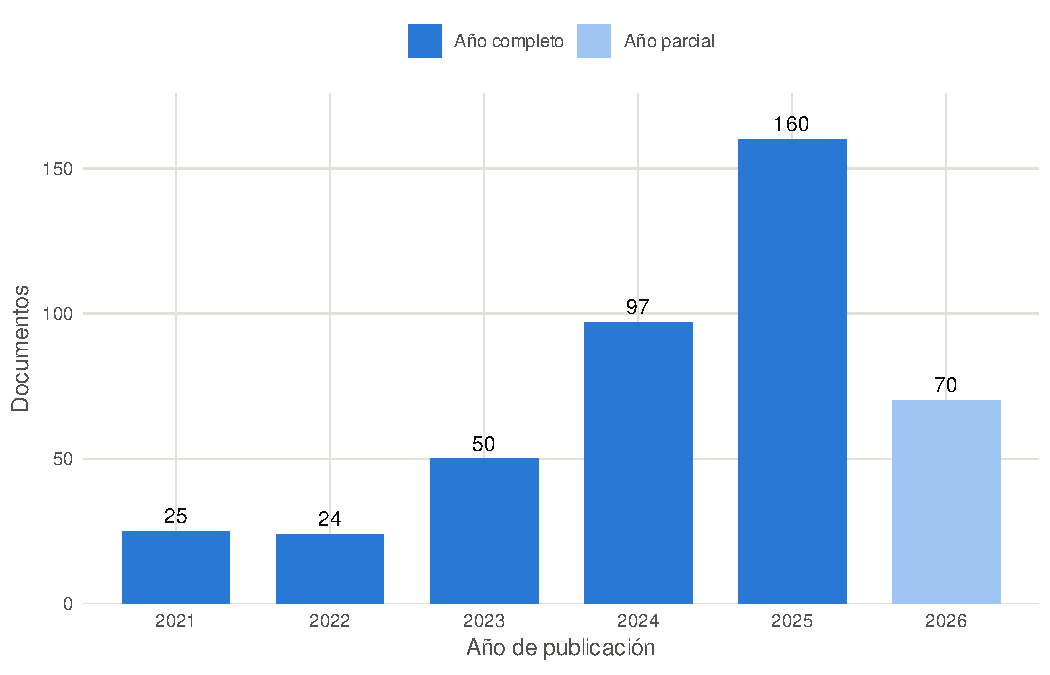
\includegraphics[width=0.75\textwidth]{ieee/es/01_annual_production}
\caption{IEEE Xplore: producción científica anual de los documentos incluidos (2026 es un año parcial, hasta el 28 de septiembre).}
\label{fig:ieee-prod}
\end{figure}

\begin{figure}[htbp]
\centering
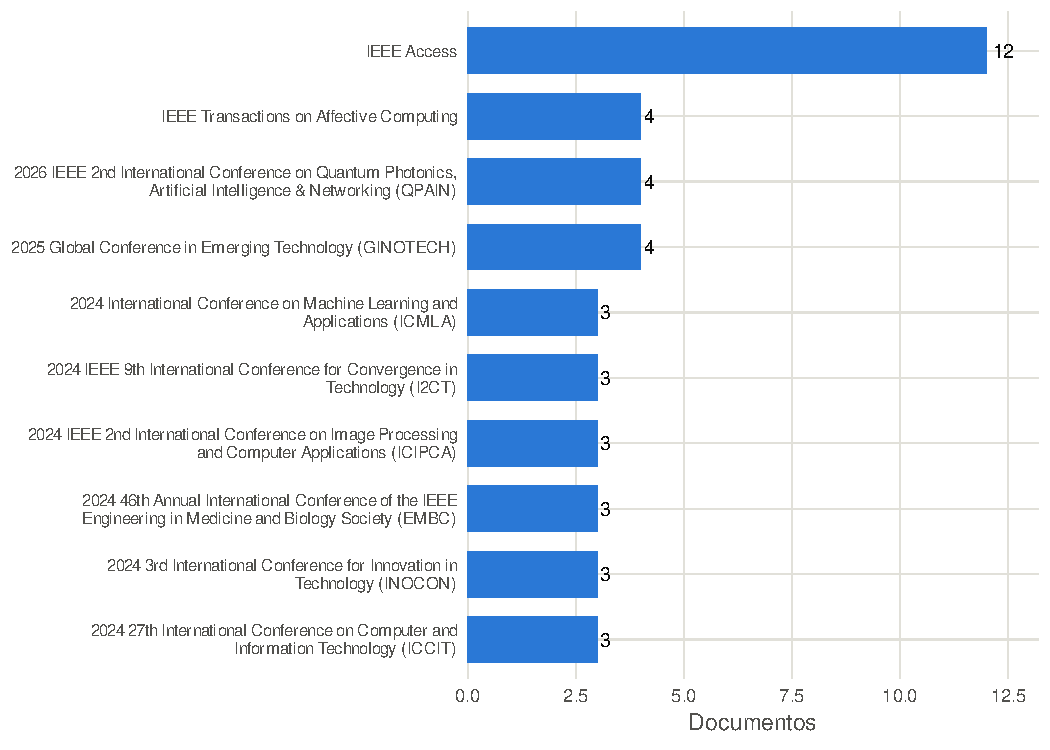
\includegraphics[width=0.85\textwidth]{ieee/es/02_sources}
\caption{IEEE Xplore: las diez fuentes más relevantes.}
\label{fig:ieee-sources}
\end{figure}

\begin{figure}[htbp]
\centering
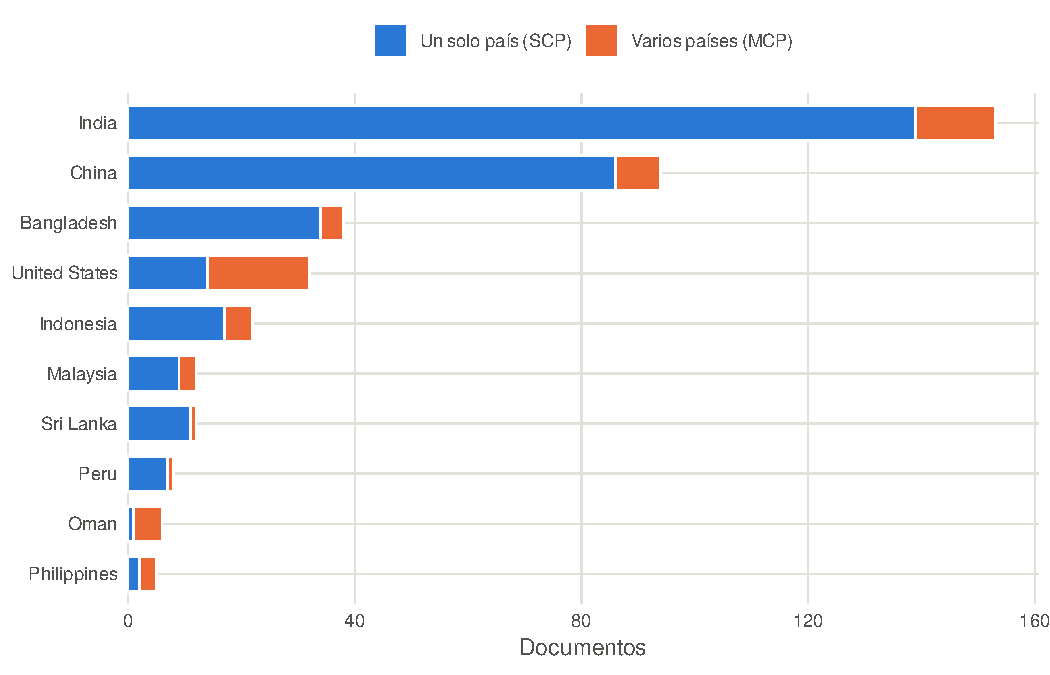
\includegraphics[width=0.75\textwidth]{ieee/es/03_countries}
\caption{IEEE Xplore: países más productivos (todos los autores, conteo completo), divididos en publicaciones de un solo país (SCP) y de varios países (MCP).}
\label{fig:ieee-countries}
\end{figure}

\begin{figure}[htbp]
\centering
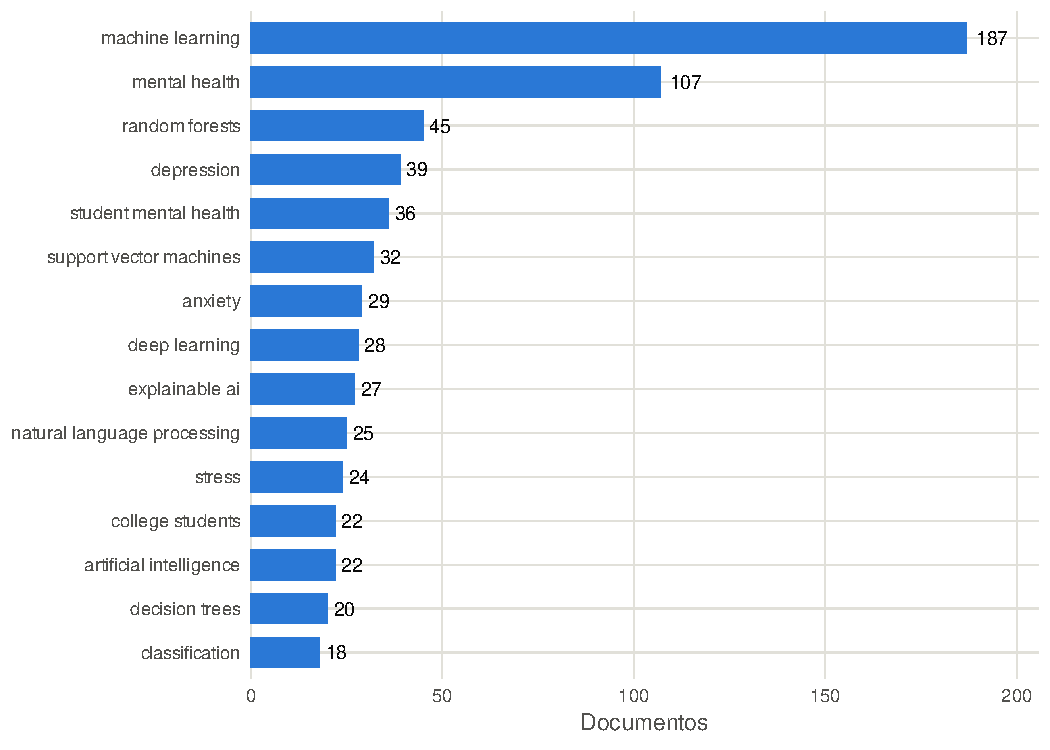
\includegraphics[width=0.75\textwidth]{ieee/es/04_keywords}
\caption{IEEE Xplore: palabras clave de autor más frecuentes (en inglés, como en los metadatos originales).}
\label{fig:ieee-keywords}
\end{figure}

\begin{figure}[htbp]
\centering
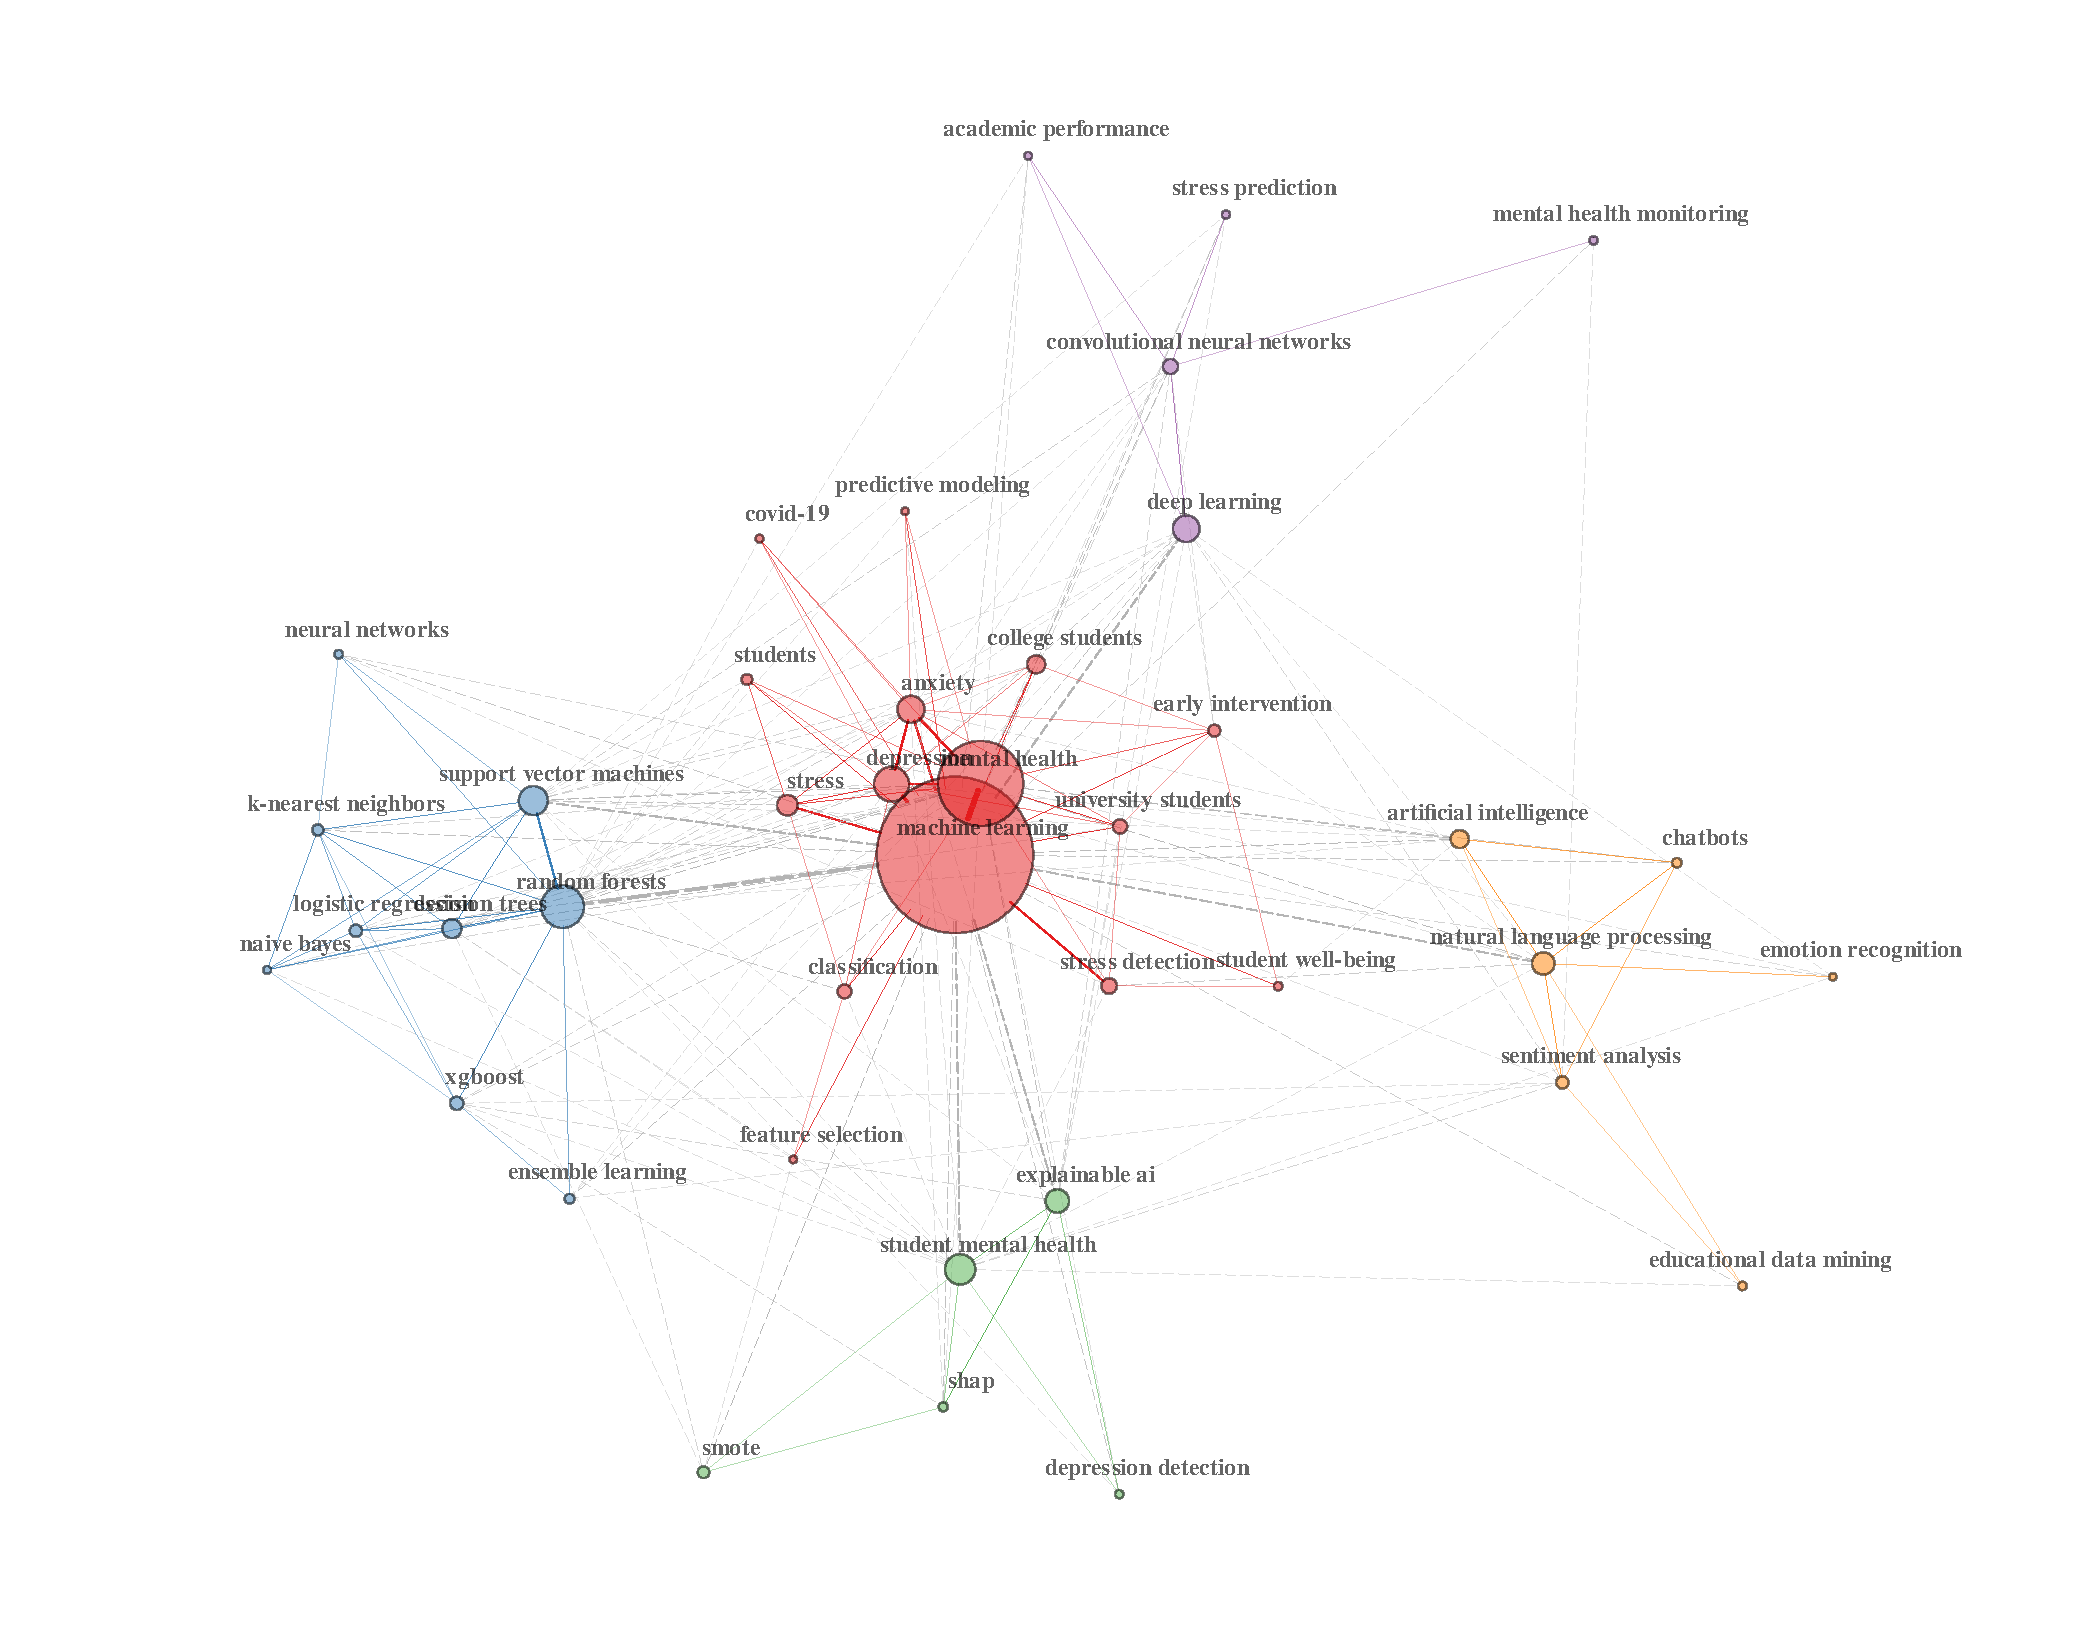
\includegraphics[width=\textwidth]{ieee/es/05_cooccurrence_network}
\caption{IEEE Xplore: red de co-ocurrencia de las 40 palabras clave de autor más frecuentes (grupos de Louvain).}
\label{fig:ieee-network}
\end{figure}

\begin{figure}[htbp]
\centering
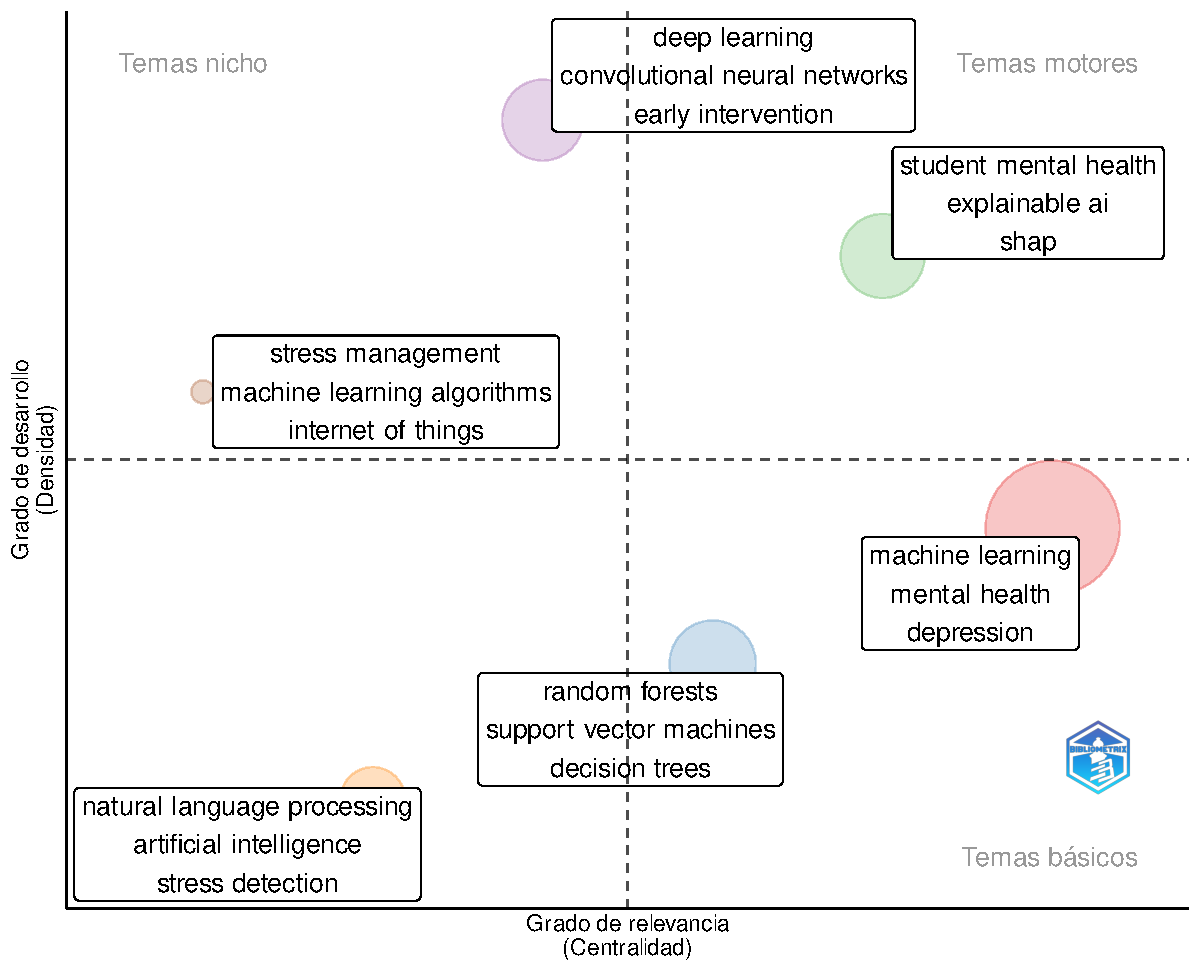
\includegraphics[width=0.85\textwidth]{ieee/es/06_thematic_map}
\caption{IEEE Xplore: mapa temático de las palabras clave de autor (centralidad frente a densidad). Cuadrantes: temas motores (arriba a la derecha), temas nicho (arriba a la izquierda), temas emergentes o en declive (abajo a la izquierda) y temas básicos (abajo a la derecha).}
\label{fig:ieee-thematic}
\end{figure}

\begin{figure}[htbp]
\centering
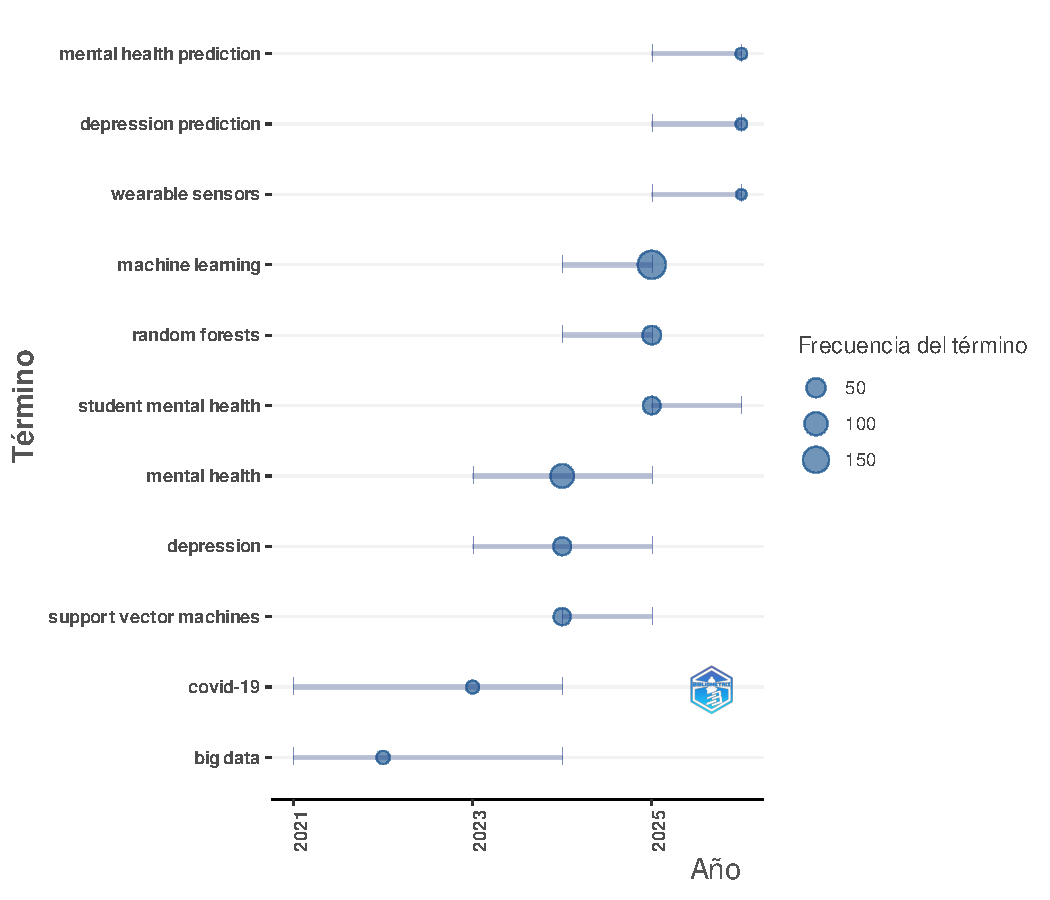
\includegraphics[width=0.75\textwidth]{ieee/es/07_trend_topics}
\caption{IEEE Xplore: tendencia de temas según el año mediano de uso.}
\label{fig:ieee-trend}
\end{figure}

\subsection{ScienceDirect}

ScienceDirect aporta 33 documentos incluidos (28 artículos de revista y 5 artículos de congreso). El análisis de palabras clave usa los conceptos de OpenAlex (33 de 33 documentos), que se asignan automáticamente y describen disciplinas; no son directamente comparables con las palabras clave de autor.

\paragraph{Producción anual.} La producción pasó de 2 documentos en 2022 a 10 en 2025, y los 10 documentos del año parcial 2026 ya igualan a 2025 (Figura~\ref{fig:sd-prod}). No se incluyó ningún registro de 2021: los cuatro registros de 2021 obtenidos no estaban relacionados con el tema. Los valores absolutos son pequeños, por lo que no se calcula una tasa de crecimiento.

\paragraph{Fuentes.} Los 33 documentos aparecen en 17 fuentes, y las tres más productivas reúnen 15 documentos (45\%) (Figura~\ref{fig:sd-sources}). Representan tres áreas: psicología (Acta Psychologica, 6), computación (Procedia Computer Science, 5) y ciencia multidisciplinar (Heliyon, 4). Las fuentes están mucho menos dispersas que en IEEE Xplore.

\paragraph{Países.} 32 documentos tienen país. China encabeza con 8 documentos, seguida de Bangladés (5), India (4), Estados Unidos (3) y España (3) (Figura~\ref{fig:sd-countries}). Tres países europeos (España, Italia y Bélgica) aparecen entre los diez más productivos, mientras que ninguno aparece entre los diez más productivos de IEEE Xplore. Solo 3 documentos (9\%) tienen autores de más de un país. Los conteos son pequeños y deben leerse como indicativos.

\paragraph{Palabras clave.} Los conceptos más frecuentes son \emph{computer science} y \emph{psychology} (17 documentos cada uno, 52\%), seguidos de \emph{machine learning} (14), \emph{mental health} (13), \emph{artificial intelligence} (12) y \emph{psychiatry} (11) (Figura~\ref{fig:sd-keywords}). El perfil es el de la intersección entre computación y psicología. En los 86 registros obtenidos antes del cribado, \emph{medicine} aparecía en 20 documentos y \emph{psychiatry} en 18; entre los 33 documentos incluidos aparecen en 6 y 11. Gran parte del aparente perfil médico de esta base provenía, por tanto, de registros no relacionados con estudiantes.

\paragraph{Gráficas excluidas.} No se incluyen la red de co-ocurrencia, el mapa temático ni la tendencia de temas. Con 33 documentos, los nodos centrales de la red se superponen, varios conceptos de OpenAlex son errores de desambiguación (por ejemplo ``classifier (UML)'' o ``feature (linguistics)''), y varios temas se apoyan en muy pocas apariciones.

\begin{figure}[htbp]
\centering
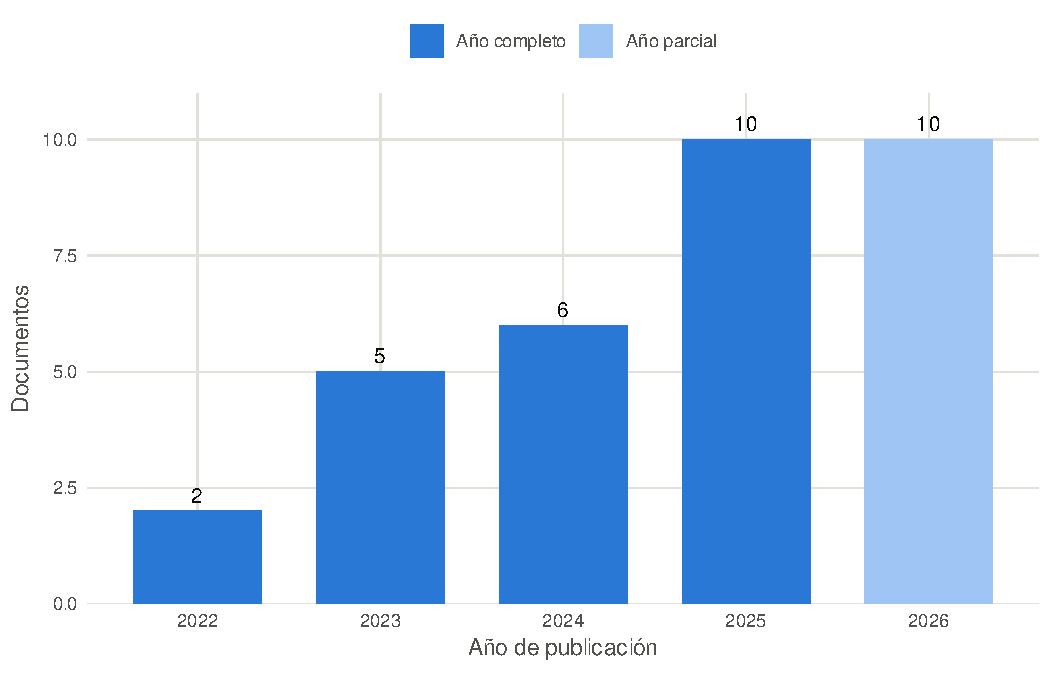
\includegraphics[width=0.7\textwidth]{sciencedirect/es/01_annual_production}
\caption{ScienceDirect: producción científica anual de los documentos incluidos (2026 es un año parcial).}
\label{fig:sd-prod}
\end{figure}

\begin{figure}[htbp]
\centering
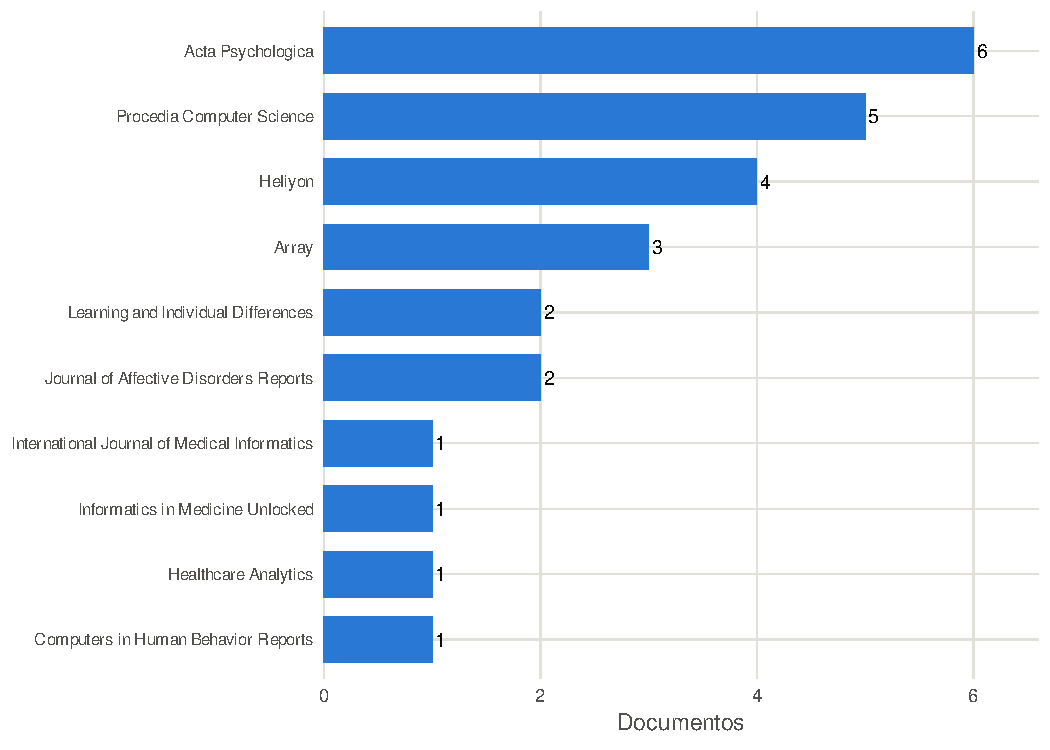
\includegraphics[width=0.8\textwidth]{sciencedirect/es/02_sources}
\caption{ScienceDirect: las diez fuentes más relevantes.}
\label{fig:sd-sources}
\end{figure}

\begin{figure}[htbp]
\centering
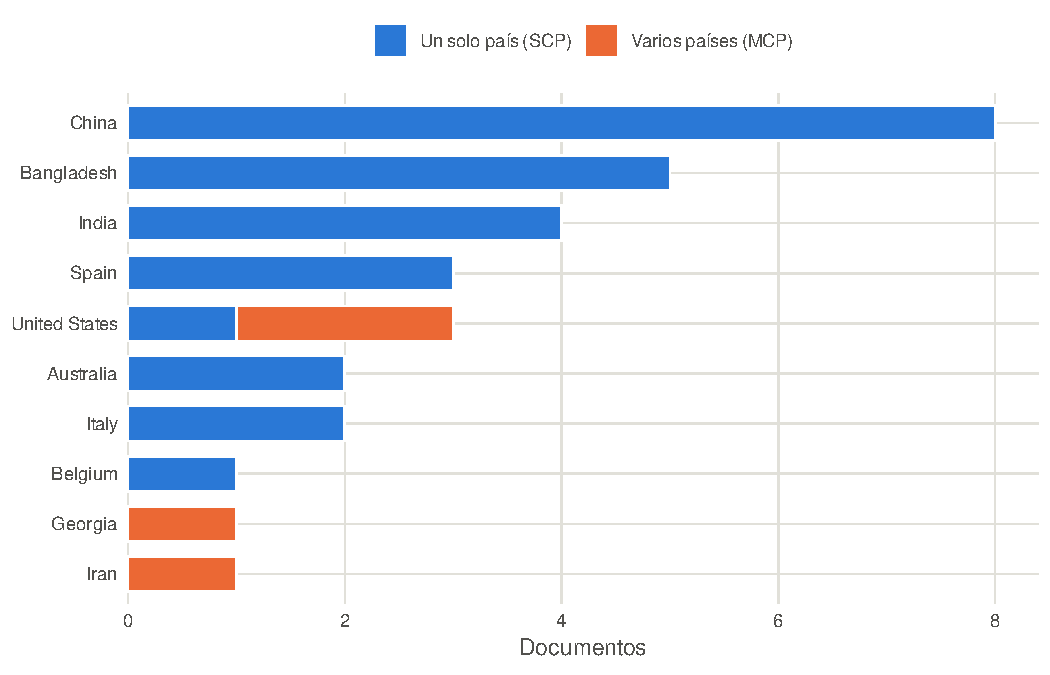
\includegraphics[width=0.7\textwidth]{sciencedirect/es/03_countries}
\caption{ScienceDirect: países más productivos (todos los autores, conteo completo).}
\label{fig:sd-countries}
\end{figure}

\begin{figure}[htbp]
\centering
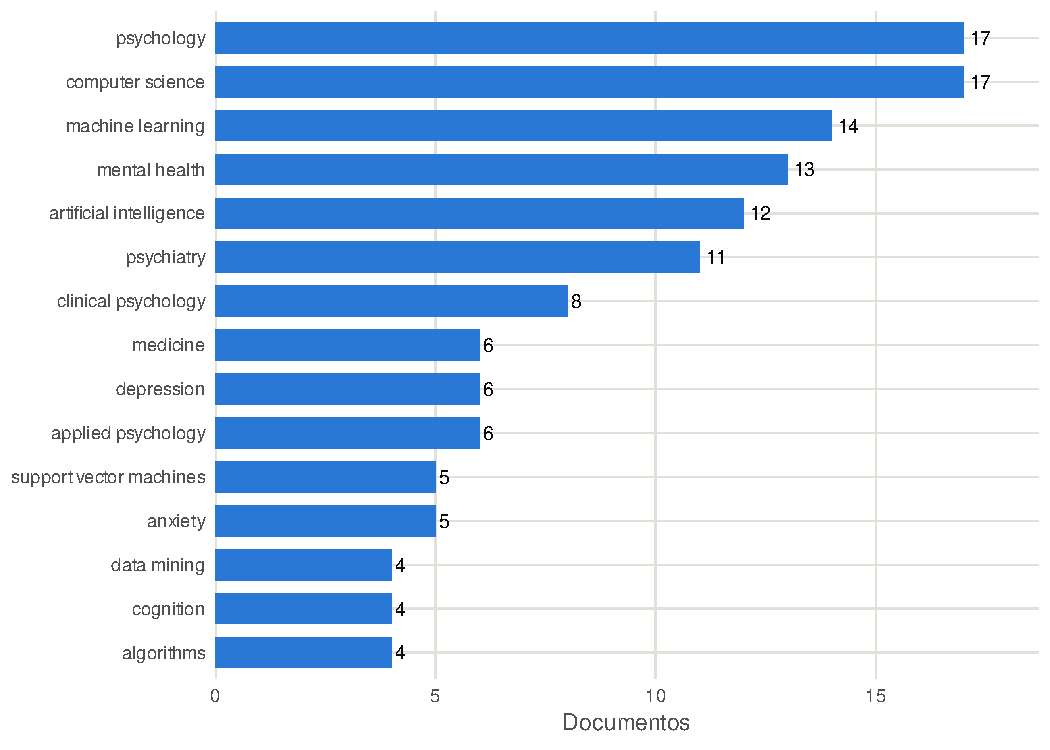
\includegraphics[width=0.7\textwidth]{sciencedirect/es/04_keywords}
\caption{ScienceDirect: conceptos de OpenAlex más frecuentes (en inglés, como en los metadatos originales).}
\label{fig:sd-keywords}
\end{figure}

\subsection{SpringerLink}

SpringerLink aporta 43 documentos incluidos (19 artículos de revista y 24 artículos de congreso), todos con palabras clave de autor. Como en SpringerLink se buscó en el campo de palabras clave, todos los documentos contienen por construcción términos de la búsqueda entre sus palabras clave.

\paragraph{Producción anual.} La producción crece cada año: 1 documento en 2021 y en 2022, 4 en 2023, 7 en 2024 y 12 en 2025 (Figura~\ref{fig:sl-prod}). Los 18 documentos del año parcial 2026 ya superan a 2025. No se calcula una tasa de crecimiento porque un valor inicial de un documento da una cifra sin sentido.

\paragraph{Países.} 36 documentos tienen país. China reúne casi la mitad (17 documentos, 47\%), seguida de India (5) y Estados Unidos (4) (Figura~\ref{fig:sl-countries}). La proporción de documentos de varios países (8 de 36, 22\%) es la más alta de las tres bases; Estados Unidos, Hong Kong, Bangladés y Canadá publican principalmente en colaboración. México (2 documentos) es el único país latinoamericano entre los diez más productivos.

\paragraph{Palabras clave.} \emph{Machine learning} aparece en el 63\% de los documentos (27 de 43) y \emph{mental health} en 18, en parte porque la búsqueda se hizo sobre este campo (Figura~\ref{fig:sl-keywords}). Lo distintivo de esta base es el vocabulario del bienestar positivo: \emph{student well-being} (4), \emph{subjective well-being} (4) y \emph{eudaimonic well-being} (2).

\paragraph{Red de co-ocurrencia.} La red tiene tres grupos (Figura~\ref{fig:sl-network}). El grupo rojo vincula \emph{machine learning} y \emph{mental health} con los estudiantes universitarios, la depresión y la detección temprana. El grupo verde reúne el bienestar subjetivo y eudaimónico, la satisfacción con la vida y PISA 2018, y se conecta con \emph{machine learning} solo mediante vínculos débiles. El grupo azul, \emph{student well-being} con \emph{learning analytics}, está aislado del resto. En esta base, el bienestar positivo se estudia en paralelo con la predicción de problemas de salud mental, no integrado con ella.

\paragraph{Gráficas excluidas.} No se incluyen la gráfica de fuentes, el mapa temático ni la tendencia de temas. Los 43 documentos se reparten en 35 fuentes y ninguna tiene más de 4 documentos; la mayoría de los temas del mapa temático se apoyan en dos apariciones de un término, y hay muy pocos términos repetidos por año para obtener tendencias confiables.

\begin{figure}[htbp]
\centering
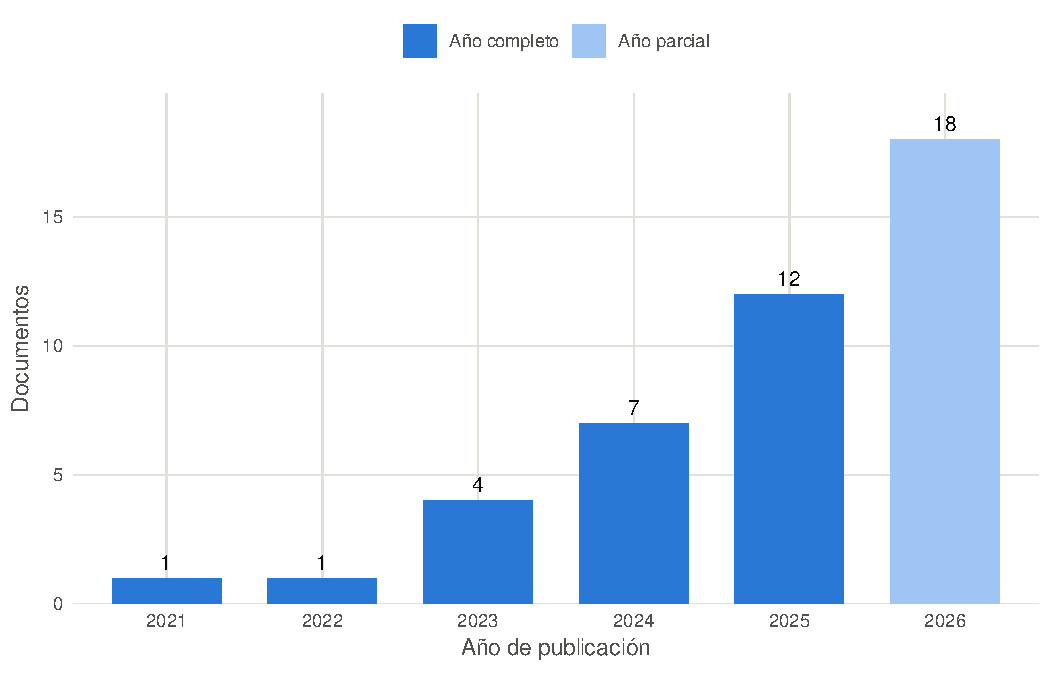
\includegraphics[width=0.7\textwidth]{springerlink/es/01_annual_production}
\caption{SpringerLink: producción científica anual de los documentos incluidos (2026 es un año parcial).}
\label{fig:sl-prod}
\end{figure}

\begin{figure}[htbp]
\centering
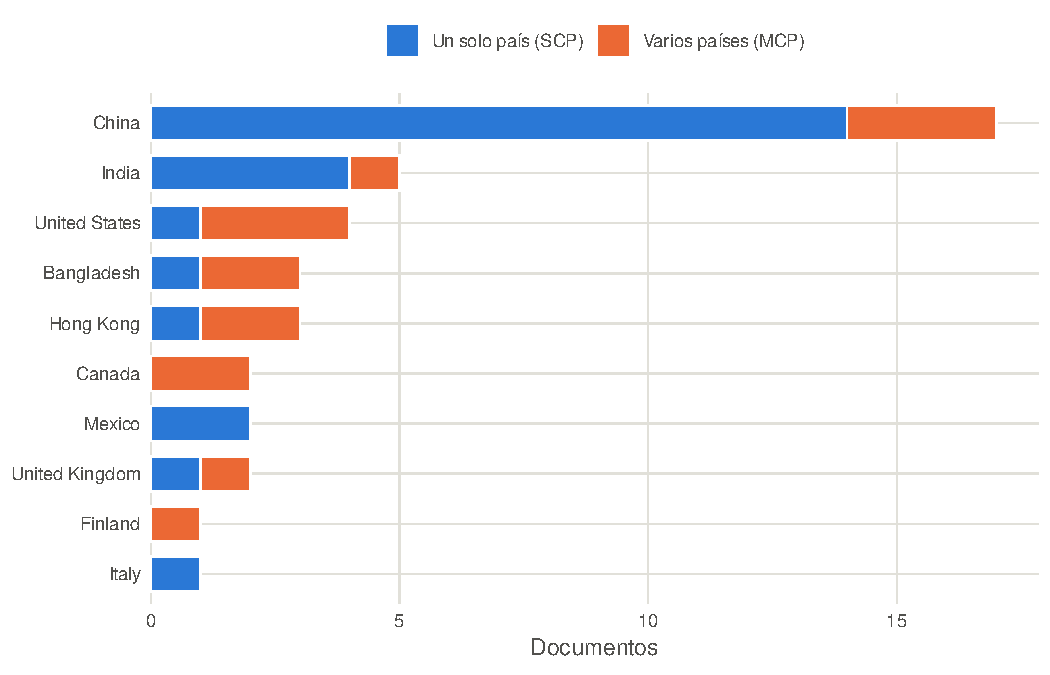
\includegraphics[width=0.7\textwidth]{springerlink/es/03_countries}
\caption{SpringerLink: países más productivos (todos los autores, conteo completo).}
\label{fig:sl-countries}
\end{figure}

\begin{figure}[htbp]
\centering
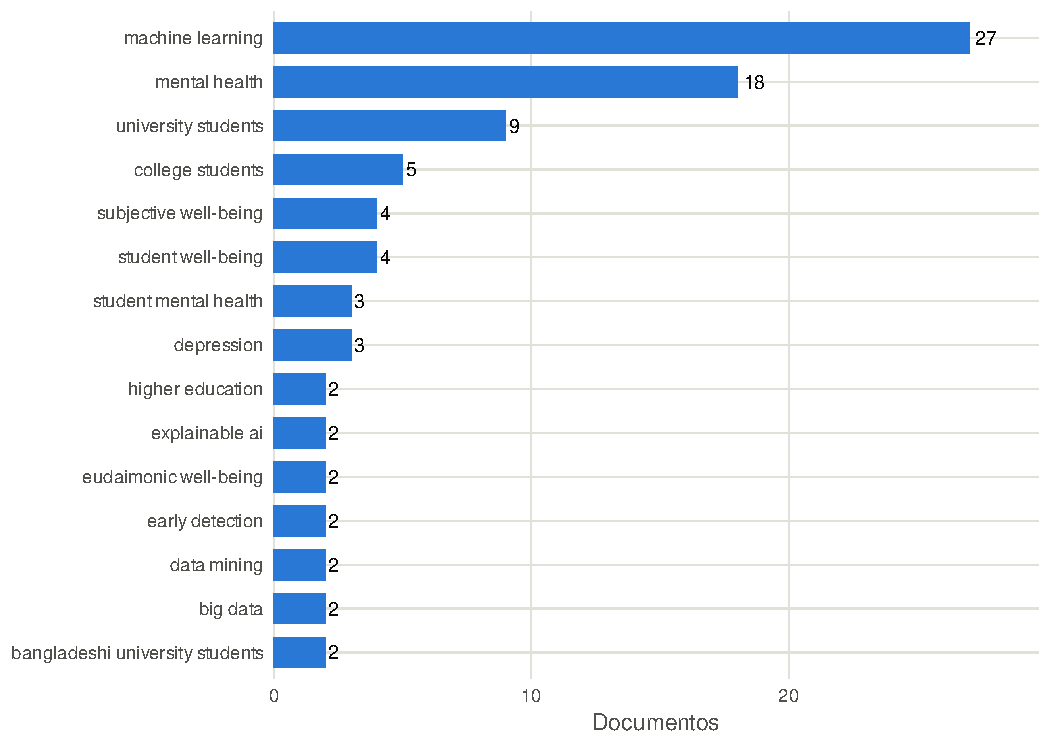
\includegraphics[width=0.7\textwidth]{springerlink/es/04_keywords}
\caption{SpringerLink: palabras clave de autor más frecuentes (en inglés, como en los metadatos originales).}
\label{fig:sl-keywords}
\end{figure}

\begin{figure}[htbp]
\centering
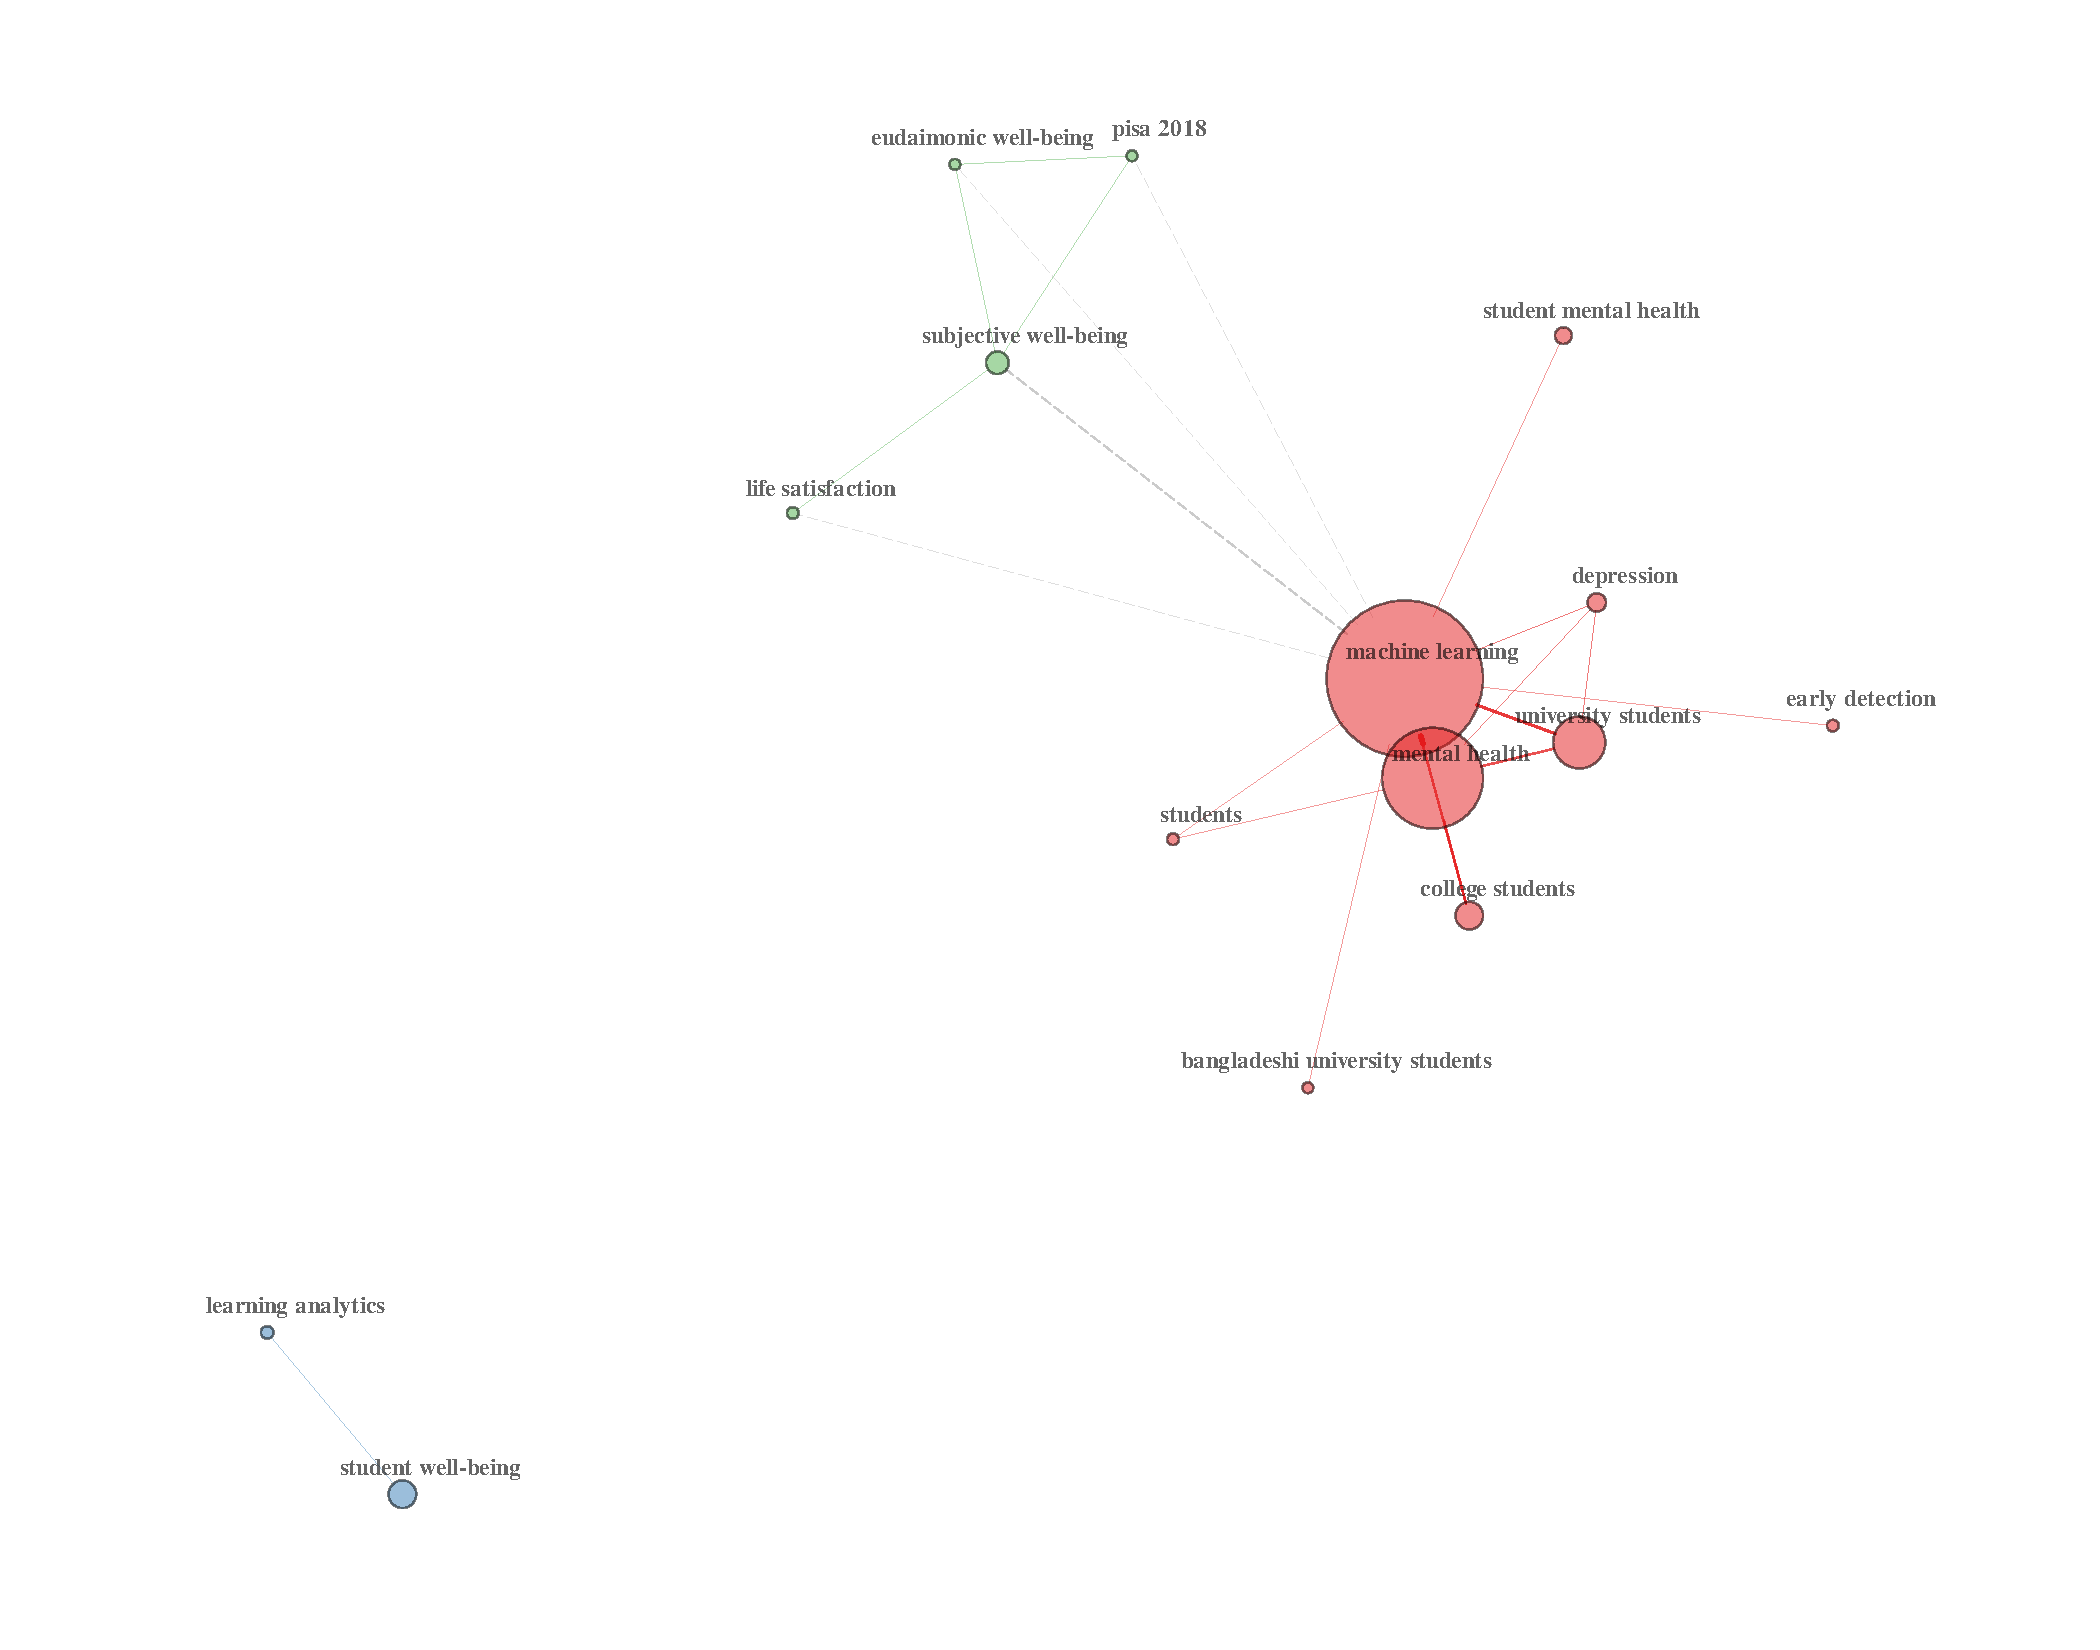
\includegraphics[width=0.9\textwidth]{springerlink/es/05_cooccurrence_network}
\caption{SpringerLink: red de co-ocurrencia de las palabras clave de autor (grupos de Louvain).}
\label{fig:sl-network}
\end{figure}

% =====================================================================
\section{Comparación entre bases de datos}\label{sec:comparison}

La Tabla~\ref{tab:comparison} resume los indicadores principales. La producción crece en las tres bases, pero difieren en volumen, tipo de documento, geografía y énfasis temático. IEEE Xplore concentra el trabajo en modelos predictivos, sobre todo en artículos de congreso. ScienceDirect, una vez eliminados los registros no relacionados, refleja la intersección entre psicología y computación en revistas. SpringerLink aporta la perspectiva del bienestar positivo. Las bases bibliográficas difieren en las disciplinas que cubren \cite{mongeon2016coverage}, y en las tres bases se buscó en campos distintos, por lo que estas diferencias reflejan también las bases y la búsqueda, no solo el campo de investigación.

\begin{table}[htbp]
\centering
\caption{Indicadores principales de los documentos incluidos por base de datos.}
\label{tab:comparison}
\small
\begin{tabularx}{\textwidth}{lYYY}
\toprule
Indicador & IEEE Xplore & ScienceDirect & SpringerLink \\
\midrule
Registros cribados / incluidos & 933 / 426 (46\%) & 86 / 33 (38\%) & 53 / 43 (81\%) \\
Artículos de revista / de congreso & 21 / 405 & 28 / 5 & 19 / 24 \\
Producción 2021 $\rightarrow$ 2025 & 25 $\rightarrow$ 160 (TCAC 59.1\%) & 0 $\rightarrow$ 10 & 1 $\rightarrow$ 12 \\
Fuentes distintas & 342 & 17 & 35 \\
Países principales & India 153, China 94, Bangladés 38 & China 8, Bangladés 5, India 4 & China 17, India 5, Estados Unidos 4 \\
Documentos de varios países & 11.7\% & 9.4\% & 22.2\% \\
Campo de palabras clave & Palabras clave de autor & Conceptos de OpenAlex & Palabras clave de autor \\
Temas distintivos & Clasificadores clásicos, aprendizaje profundo, XAI, PLN & Psicología y computación & Bienestar subjetivo y eudaimónico \\
Resúmenes vagos & 43\% & 9\% & 21\% \\
XAI reportada & 10\% & 33\% & 23\% \\
\bottomrule
\end{tabularx}
\end{table}

% =====================================================================
\section{Discusión}\label{sec:discussion}

\subsection{Respuestas a las preguntas de investigación}

\textbf{PI1 (evolución).} La producción creció en las tres bases entre 2021 y 2025, a una tasa anual compuesta del 59.1\% en IEEE Xplore. Con 2026 aún incompleto, su producción ya supera la de 2023 en IEEE Xplore (70 frente a 50), iguala la de 2025 en ScienceDirect (10) y supera la de 2025 en SpringerLink (18 frente a 12).

\textbf{PI2 (países).} India, China y Bangladés encabezan la producción. Los países indicados en los resúmenes apuntan en la misma dirección: Bangladés (27 estudios), China (20) e India (17) son los más frecuentes. La colaboración internacional es baja (entre el 9.4\% y el 22.2\% de los documentos), y los dos países más productivos publican casi siempre sin socios extranjeros. América Latina tiene una presencia marginal (Perú y México).

\textbf{PI3 (fuentes).} La investigación se publica principalmente en actas de congresos y está muy dispersa, sobre todo en IEEE Xplore, donde 342 fuentes se reparten 426 documentos. Solo ScienceDirect muestra cierta concentración en revistas (Acta Psychologica, Procedia Computer Science, Heliyon).

\textbf{PI4 (resultados, poblaciones, datos y técnicas).} El campo se organiza alrededor de la predicción del estrés, la depresión y la ansiedad en estudiantes universitarios, principalmente a partir de cuestionarios y con clasificadores clásicos y ensambles de árboles. Los enfoques basados en sensores, en texto y multimodales forman líneas secundarias. El suicidio, los estudiantes de secundaria y el bienestar positivo reciben comparativamente poca atención.

\textbf{PI5 (cambio en el tiempo).} El vocabulario pasa de términos de contexto (\emph{big data}, COVID-19) a la predicción y, más recientemente, a la predicción con sensores vestibles. El contenido codificado muestra la misma dirección: aumentó la proporción de estudios que usan aprendizaje profundo y XAI, y la XAI pasó del 4\% al 32\%.

\textbf{PI6 (énfasis de cada base).} IEEE Xplore muestra el modelado predictivo, ScienceDirect la intersección entre psicología y computación, y SpringerLink el bienestar positivo. Como IEEE Xplore aporta el 85\% de los documentos incluidos, las conclusiones generales reflejan sobre todo esa base.

\subsection{Vacíos}

El principal vacío es metodológico. La validación con una cohorte externa se reporta solo en dos resúmenes, la calibración en tres y la equidad en siete, mientras que al menos 44 estudios reportan valores de desempeño del 98\% o más. Las muestras pequeñas con una validación inadecuada inflan las estimaciones de desempeño \cite{vabalas2019validation}, y la fuga de información es una causa frecuente de resultados no reproducibles \cite{kapoor2023leakage}. Ningún resumen menciona una guía de reporte como TRIPOD+AI \cite{collins2024tripodai}, y el 26\% de los resúmenes no indica los datos usados.

El uso de XAI está creciendo, pero explicar un modelo complejo después de entrenarlo no equivale a usar un modelo interpretable por diseño, y para decisiones de alto impacto son preferibles los modelos interpretables \cite{rudin2019blackbox}. El tamizaje de problemas de salud mental en estudiantes es una decisión de alto impacto: un falso negativo puede dejar a un estudiante en riesgo sin apoyo, y por eso algunos estudios del corpus priorizan la sensibilidad (\emph{recall}) \cite{S008}.

En lo temático, el bienestar positivo y la predicción de problemas de salud mental se estudian en paralelo, como muestra la red de SpringerLink. El suicidio aparece solo en el 3\% de los estudios y los estudiantes de secundaria en el 5\%. La privacidad o la confidencialidad se mencionan en 39 resúmenes (8\%), en general como una característica del diseño o una preocupación ética y no como el objeto del estudio.

\subsection{Agenda de investigación futura}

A partir de estos vacíos, la investigación futura debería: (i) validar los modelos con datos independientes, entre instituciones y en el tiempo; (ii) reportar los estudios según TRIPOD+AI \cite{collins2024tripodai}, incluyendo la fuente de datos, el tamaño de la muestra, el manejo del desbalance de clases y la calibración; (iii) preferir modelos interpretables o evaluar las explicaciones con sus usuarios, como los orientadores; (iv) conectar los constructos de bienestar positivo con la predicción de problemas de salud mental; (v) evaluar si los sistemas de alerta temprana mejoran los resultados de los estudiantes, y no solo si clasifican con exactitud; (vi) abordar de forma explícita la equidad, el consentimiento y la privacidad; y (vii) extender la evidencia a la educación secundaria y a regiones con poca presencia en el corpus, como América Latina.

% =====================================================================
\section{Limitaciones}\label{sec:limitations}

Este estudio tiene varias limitaciones. Primero, el corpus proviene de tres bases consultadas mediante sus API con campos de búsqueda distintos: en SpringerLink solo se buscó en las palabras clave, y los registros de ScienceDirect se obtuvieron a través de Scopus. Pueden faltar estudios pertinentes indexados en otras bases o descritos solo en el texto completo. Segundo, las bases están desbalanceadas: IEEE Xplore aporta el 85\% de los documentos incluidos. Tercero, el cribado y la extracción de datos se basaron solo en los resúmenes y se hicieron con la asistencia de un modelo de lenguaje de gran tamaño bajo un libro de códigos cerrado, seguidos de verificaciones sobre muestras aleatorias, verificaciones dirigidas de las decisiones dudosas y reglas de armonización documentadas; no se realizó una doble codificación independiente completa por revisores humanos. Cuarto, las API no entregan las listas de referencias, por lo que no fueron posibles los análisis basados en citas (co-citación, acoplamiento bibliográfico, referencias más citadas). Quinto, las palabras clave de ScienceDirect son conceptos de OpenAlex asignados automáticamente, que no son comparables con las palabras clave de autor y contienen errores de desambiguación. Sexto, 2026 es un año parcial, y el número de citas y los campos de OpenAlex cambian con el tiempo; todos los resultados se refieren a la captura del 28 de septiembre de 2026. Por último, solo se analizaron registros en inglés.

% =====================================================================
\section{Conclusiones}\label{sec:conclusions}

Este estudio combinó una revisión sistemática de 502 resúmenes con un análisis bibliométrico comparativo de IEEE Xplore, ScienceDirect y SpringerLink para mapear la analítica del bienestar y la salud mental estudiantil entre 2021 y 2026. El campo crece con rapidez y se concentra en India, China y Bangladés. Se organiza alrededor de la predicción del estrés, la depresión y la ansiedad en estudiantes universitarios a partir de cuestionarios, con clasificadores clásicos y ensambles de árboles, y avanza hacia el aprendizaje profundo, los modelos de lenguaje, los sensores vestibles y los modelos explicables.

Cribar los resúmenes cambió el panorama: casi un tercio de los registros obtenidos no estaba relacionado con el tema, y eliminarlos cambió el perfil aparente de ScienceDirect. La principal debilidad del campo es la distancia entre el alto desempeño que reportan los estudios y la débil validación que lo respalda. El avance depende ahora de la validación con datos independientes, el reporte transparente, los modelos interpretables y la evidencia de que los sistemas de alerta temprana ayudan a los estudiantes.

% =====================================================================
\section*{Declaraciones}

\paragraph{Disponibilidad de los datos.} Las ecuaciones de búsqueda, los scripts de obtención y de análisis, el libro de códigos, los registros cribados y codificados (con sus identificadores y DOI) y el registro de armonización están disponibles en acceso abierto en \url{https://github.com/lyc4nthrope/student-wellbeing-mental-health-analytics-review}. Los resúmenes de las editoriales no se redistribuyen; pueden obtenerse de nuevo con el script de obtención y las claves de API propias del lector.

\paragraph{Uso de inteligencia artificial.} Se usó un modelo de lenguaje de gran tamaño como apoyo en el cribado de resúmenes, la extracción de datos y la redacción de este manuscrito. El autor revisó los resultados y es responsable del contenido.

\bibliographystyle{unsrtnat}
\bibliography{references,corpus}

\end{document}
